% Options for packages loaded elsewhere
\PassOptionsToPackage{unicode}{hyperref}
\PassOptionsToPackage{hyphens}{url}
%
\documentclass[
  11pt,
]{article}
\usepackage{amsmath,amssymb}
\usepackage{lmodern}
\usepackage{iftex}
\ifPDFTeX
  \usepackage[T1]{fontenc}
  \usepackage[utf8]{inputenc}
  \usepackage{textcomp} % provide euro and other symbols
\else % if luatex or xetex
  \usepackage{unicode-math}
  \defaultfontfeatures{Scale=MatchLowercase}
  \defaultfontfeatures[\rmfamily]{Ligatures=TeX,Scale=1}
\fi
% Use upquote if available, for straight quotes in verbatim environments
\IfFileExists{upquote.sty}{\usepackage{upquote}}{}
\IfFileExists{microtype.sty}{% use microtype if available
  \usepackage[]{microtype}
  \UseMicrotypeSet[protrusion]{basicmath} % disable protrusion for tt fonts
}{}
\makeatletter
\@ifundefined{KOMAClassName}{% if non-KOMA class
  \IfFileExists{parskip.sty}{%
    \usepackage{parskip}
  }{% else
    \setlength{\parindent}{0pt}
    \setlength{\parskip}{6pt plus 2pt minus 1pt}}
}{% if KOMA class
  \KOMAoptions{parskip=half}}
\makeatother
\usepackage{xcolor}
\usepackage[margin=1.0in]{geometry}
\usepackage{graphicx}
\makeatletter
\def\maxwidth{\ifdim\Gin@nat@width>\linewidth\linewidth\else\Gin@nat@width\fi}
\def\maxheight{\ifdim\Gin@nat@height>\textheight\textheight\else\Gin@nat@height\fi}
\makeatother
% Scale images if necessary, so that they will not overflow the page
% margins by default, and it is still possible to overwrite the defaults
% using explicit options in \includegraphics[width, height, ...]{}
\setkeys{Gin}{width=\maxwidth,height=\maxheight,keepaspectratio}
% Set default figure placement to htbp
\makeatletter
\def\fps@figure{htbp}
\makeatother
\setlength{\emergencystretch}{3em} % prevent overfull lines
\providecommand{\tightlist}{%
  \setlength{\itemsep}{0pt}\setlength{\parskip}{0pt}}
\setcounter{secnumdepth}{5}
\newcommand{\bcenter}{\begin{center}}
\newcommand{\ecenter}{\end{center}}
\newcommand{\btitlepage}{\begin{titlepage}}
\newcommand{\etitlepage}{\end{titlepage}}
\usepackage{helvet}
\renewcommand*\familydefault{\sfdefault}
\usepackage{setspace}\doublespacing
\usepackage{booktabs}
\usepackage[font=small,labelfont=bf]{caption}
\usepackage{array}
\usepackage{setspace}
\newcommand{\blandscape}{\begin{landscape}}
\newcommand{\elandscape}{\end{landscape}}
\usepackage{booktabs}
\usepackage{longtable}
\usepackage{array}
\usepackage{multirow}
\usepackage{wrapfig}
\usepackage{float}
\usepackage{colortbl}
\usepackage{pdflscape}
\usepackage{tabu}
\usepackage{threeparttable}
\usepackage{threeparttablex}
\usepackage[normalem]{ulem}
\usepackage{makecell}
\usepackage{xcolor}
\ifLuaTeX
  \usepackage{selnolig}  % disable illegal ligatures
\fi
\IfFileExists{bookmark.sty}{\usepackage{bookmark}}{\usepackage{hyperref}}
\IfFileExists{xurl.sty}{\usepackage{xurl}}{} % add URL line breaks if available
\urlstyle{same} % disable monospaced font for URLs
\hypersetup{
  hidelinks,
  pdfcreator={LaTeX via pandoc}}

\author{}
\date{\vspace{-2.5em}}

\begin{document}

\begin{titlepage}

\begin{center}

\vspace*{30mm}

Candidate number: 49045

\vspace*{10mm}

\hypertarget{title-here}{%
\section*{TITLE HERE}\label{title-here}}
\addcontentsline{toc}{section}{TITLE HERE}

\vspace*{10mm}

Supervisor: Ekaterina (Katya) Oparina\\

Word count:

\vspace*{30mm}

Submitted as partial fulfilment for\\

MSc in Behavioural Science\\

Department of Psychological and Behavioural Science\\

The London School of Economics and Political Science

\end{center}

\end{titlepage}

\newpage

Total word limit: 10000

\hypertarget{abstract-100-150}{%
\section*{Abstract (100-150)}\label{abstract-100-150}}
\addcontentsline{toc}{section}{Abstract (100-150)}

\newpage

\hypertarget{introduction-1000}{%
\section*{Introduction (1000)}\label{introduction-1000}}
\addcontentsline{toc}{section}{Introduction (1000)}

Gender gap in labour force participation is a world-wide phenomenon
which is particularly pronounced in developing countries. Globally, the
rate of labour force participation is about 75\% among men while only
50\% among women \textbf{(International Labour Organization, 2021)}. In
regions such as Middle East, North Africa, and South Asia, the gender
gap is even greater, with around 75\% of men and 20\% of women
participating in the labour force \textbf{(International Labour
Organization, 2021)}. In search of potential measures to narrow the
gender gap, its causes have been extensively studied with a recent
attention to the prominent role of social norms. Researchers speculate
that interventions aiming at changing social norms may be the key to
achieve greater gender equality in labour force participation
\textbf{(Bursztyn et al., 2020; Codazzi et al., 2018; Jayachandran,
2021)}.

A recent attempt in developing such a social norm intervention was made
by Bursztyn and colleagues \textbf{(2020)} in Saudi Arabia. In Saudi
Arabia, gender norms exist that expect women to be absent from labour or
segregated from men at workplace, and that women need approval from
their male ``guardian'' (usually the husband or father) if they want to
work outside the home \textbf{(Bursztyn et al., 2018)}. These may lead
us to reasonably speculate that the low female labour participation rate
in Saudi Arabia \textbf{(28\% in 2022, International Labour
Organization)} is because men don't allow their wives to work outside
the home (WWOH) due to the internalisation of the gender norms (i.e.,
personal beliefs aligning with the norm that women should not work
outside the home). Interestingly, however, Bursztyn and colleagues
\textbf{(2020)} found that the critical factor was rather Saudi men's
misperception of the injunctive norms regarding WWOH. Their findings
revealed that 80-85\% of surveyed Saudi men who were married and aged
18-35 reported to agree with the statement that women should be allowed
to work outside the home, while more than three quarters underestimated
this percentage. This phenomenon is also referred to as pluralistic
ignorance (PI) \textbf{(Bursztyn et al., 2020)}.

Based on this finding, Bursztyn and colleagues \textbf{(2020)} designed
an intervention to correct men's misperception regarding WWOH and found
supporting evidence for its effectiveness in changing their labour
supply decisions. They found that men who received the information of
the true percentage of WWOH supporters (vs.~those who did not receive
the information) were significantly more likely to sign up for job
matching service for their wives immediately after the intervention.
Their wives were also more likely to have applied and interviewed for a
job three to five months after the intervention. The researchers also
tested the effect of a similar intervention on Saudi women in a field
setting, finding that women who received the information on the
percentage of men supporting WWOH (vs.~those who did not received the
information) were more likely to take up a part-time job outside the
home instead of a position to work at home.

Recognising the potential of correcting norm misperception as an
intervention measure to create behavioural change, the present research
aims to use computer simulations to further explore its theoretical
effectiveness when scaled up. Specifically, an agent-based model (ABM)
will be built to simulate PI regarding WWOH in Saudi Arabia and its
interventions. ABMs are a type of computational model that simulates in
a synthetic environment the actions and interactions of autonomous
agents, whose behaviours determine the evolution of the entire system
\textbf{(Bandini et al., 2009)}. ABMs are particularly suitable to model
and study dynamics and emergent properties in complex systems that are
irreducible to lower-level descriptions (e.g., mathematical equations)
\textbf{(Gustafsson \& Sternad, 2010)}. One example of such a system is
where agents interact dynamically and irregularly over time
\textbf{(Johnson, 2009; Gustafsson \& Sternad, 2010)}. The ability in
modelling multi-agent complex systems makes ABMs widely applied in
studying interventions to human behaviours in various fields. These
include but are not limited to the effect of lock-down policy in
epidemiology \textbf{(de Mooij et al., 2022)}, fishery policy in
sustainable management \textbf{(Bailey et al., 2018)}, and interventions
to the spread of misinformation \textbf{(Pilditch et al., 2022)}.

By building an ABM, the present research seeks to answer two broad
questions: under what conditions PI regarding WWOH in Saudi Arabia are
sustained and under what conditions social norm interventions can reduce
PI and encourage WWOH behaviours? The paper proceeds as follows. Section
1 reviews literature that is relevant to model-building in the present
research, including mathematical and computational models of belief and
action dynamics, ABMs of pluralistic ignorance, and empirical research
of existing social norm intervention strategies. Section 2 introduces
the details of the model and the simulation. Section 3 presents the
results. Section 4 discusses the implications of the findings and
concludes.

\hypertarget{literature-review-2000}{%
\section{Literature Review (2000)}\label{literature-review-2000}}

\hypertarget{models-of-belief-and-action-dynamics}{%
\subsection{Models of Belief and Action
Dynamics}\label{models-of-belief-and-action-dynamics}}

Pluralistic ignorance regarding WWOH as a population-level phenomenon is
underlain by complex interpersonal interactions among people's private
beliefs and public actions. One's labour supply decision and action can
presumably influence their acquaintances' private belief and norm
perception, and these influences in turn impact their acquaintances'
labour supply decision and action as a function of private belief and
norm perception. Such belief and action dynamics among interconnected
and mutually influencing individuals have been studied widely through
mathematical and computational models. These models assume that agents
hold beliefs regarding certain issues. At each time step, these beliefs
are modified based on their neighbours' beliefs according to some rules.
The dynamics of belief distribution in a population over time is
studied. This section will review formal methods to model beliefs and
actions dynamics in a population and some applications of these models,
which will serve as a basic framework for modelling PI regarding WWOH in
the present research.

Models of belief and action dynamics are characterised by different
assumptions about how agents' beliefs and actions are updated based on
those of others \textbf{(Hassani et al., 2022)}. The most simplistic
models represent agents' beliefs using binary variables, the classic
ones of which include the Ising model \textbf{(Li et al., 2019)}, the
voter model \textbf{(Holley \& Liggett, 1975)}, and the Sznajd model
\textbf{(Sznajd-Weron \& Sznajd, 2000)}. These models usually assume
that agents update beliefs by replacing them with those of their
neighbours. For example, in the voter model, an agent \(i\) is randomly
chosen at each time step, together with one of its neighbour \(j\). The
agent \(i\) then abandons its previous belief and takes up the opinion
of its neighbour \(j\). Therefore, in these simplistic models, the
updating usually results in the agents being memoryless about their
previous beliefs.

Other simple models represent agents' beliefs as continuous variables
that take the value of a real number. These are exemplified by the
classic Degroot model \textbf{(Berger, 1981)} and the bounded confidence
model \textbf{(Rainer \& Krause, 2002)}. Models of this type usually
update agents' beliefs using a weighted average of an individual's
belief and those of their neighbour(s). For example, in the bounded
confidence model, an agent \(i\) is randomly chosen at each time step
\(t\), together with one of its neighbour \(j\), who hold the beliefs
\(\sigma_i(t)\) and \(\sigma_j(t)\), respectively. When the condition
\(|\sigma_i(t) - \sigma_j(t)| < \epsilon\) is met, the agent \(i\)
updates its belief according to
\(\sigma_i(t+1) = (1 - \alpha)\sigma_i(t) + \alpha\sigma_j(t)\), and the
agent \(j\) according to
\(\sigma_j(t+1) = (1 - \alpha)\sigma_j(t) + \alpha\sigma_i(t)\). In
other words, when the selected agents hold similar enough beliefs
according to a threshold \(\epsilon\), they update their beliefs as the
weighted average of their previous beliefs based on a convergence
parameter \(\alpha\).

More sophisticated models recognise the distinction between agents'
private beliefs and public actions, modelling the former as a continuous
variable and the latter a discrete one. The Continuous Opinions and
Discrete Actions (CODA) model \textbf{(Martins, 2013)} and the recent
social network opinions and actions evolutions (SNOAEs) model
\textbf{(Zhan et al., 2022)} are examples of this category. To take the
CODA model as an example, it models private beliefs as
\(P(A) \in [0,1]\), the probability of the \(A\) being the best
alternative. Agents have no access to other agents' private beliefs but
only their public actions, which is used to update one's own private
beliefs. For example, upon observing neighbour \(j\) displaying the
action \(A\) at the time step \(t\), an agent update its private beliefs
according to the Bayes' theorem
\(P_{t+1}(A) = P(A | a_j = +1) \propto P_t(A) P(a_j = +1 | A)\), where
\(P(A | a_j = +1)\) denotes the probability of \(A\) being the best
action conditioned on the neighbour \(j\) displaying \(A\), and
\(P(a_j = +1 | A)\) the probability of the neighbour \(j\) displaying
\(A\) conditioned on \(A\) being the best action (which is modelled as a
constant).

It is important to notice that there is a recent trend to build
psychologically realistic models to represent belief and behaviour
dynamics in a population \textbf{(Duggins, 2017; Gavrilets, 2021;
Tverskoi et al., 2023)}. Apart from agents' beliefs and actions, these
models further consider the influence of social norm, the psychological
tendency to conform to peers, external authorities, as well as material
cost-benefit considerations \textbf{(Gavrilets, 2021)}. To incorporate
these psychological and social complexities, a recent unifying modelling
framework \textbf{(Gavrilets, 2021)} models agents' perception of
others' private beliefs and public actions as two variables independent
from their own beliefs and actions. This allows the representation of
various psychological factors in updating beliefs and actions, including
cognitive dissonance in taking a private belief (i.e., the aversion
towards misaligned belief and action), social projection in perceiving
others' private beliefs (i.e., the tendency to project one's own private
belief onto others), and compliance with authority.

Models of belief and action dynamics have been applied to studying
multiple themes associated with opinion change in a population. These
include but are not limited to consensus reaching and polarisation
\textbf{(Acemoglu \& Ozdaglar, 2010; Hassani et al., 2022; Jager \&
Amblard, 2004; Duggins, 2017)}, the spread of (mis)information
\textbf{(Watts, 2002; Watts \& Dodds, 2007; Pilditch et al., 2022)}, and
echo chamber formation \textbf{(Madsen et al., 2018; Fränken \&
Pilditch, 2021)}. Researchers are mostly interested in exploring the
assumptions and conditions that can give rise to certain phenomena. For
instance, a study reviews a series of mathematical models to inquire
into the belief updating mechanisms that facilitate consensus reaching,
information aggregation, and the spread of misinformation
\textbf{(Acemoglu \& Ozdaglar, 2010)}. It finds that in both Bayesian
and non-Bayesian models, there is a tendency towards reaching consensus.
Misinformation spreads with limited extent, which is due to the limited
influence of misinformation on Bayesian agents in Bayesian models, and
the lack of persistent disagreements in the population in non-Bayesian
models. Another example is a series of research that studies how
assumptions about network structures can influence information cascade,
a phenomenon where a group of individuals make the same decision
sequentially \textbf{(Watts, 2002; Watts \& Dodds, 2007)} It finds that
the distribution of the size of cascades depends on the connectivity of
the network \textbf{(Watts, 2002)}, and that influential individuals
(i.e., those who have the highest number of connections to others) are
not sufficient for triggering cascades, but the existence of a group of
individuals who are easily influenced by them is critical \textbf{(Watts
\& Dodds, 2007)}.

\hypertarget{agent-based-models-of-pluralistic-ignorance}{%
\subsection{Agent-Based Models of Pluralistic
Ignorance}\label{agent-based-models-of-pluralistic-ignorance}}

Although the discussion about pluralistic ignorance is born in
psychological research \textbf{(e.g., Prentice \& Miller, 1993)}, there
has been a growing interest in using ABMs to study the conditions under
which this phenomenon can arise. This line of research usually defines
PI as the situation where the majority of people in a population express
opinions different from their private beliefs \textbf{(e.g., Seeme et
al., 2016; Wang et al., 2014; Ye et al., 2019)}. The seminal simulation
study on this topic focuses on the effects of network properties on
holding inconsistent private beliefs and expressed opinions
\textbf{(Centola et al., 2005)}. The simulation inserts to a population
a few ``true believers'' of an unpopular norm (i.e., agents who hold a
private belief held by few individuals in the population) who enforce
other agents to adopt the belief. It reveals that the phenomenon of
holding inconsistent private beliefs and expressed opinions cannot
spread widely in the population if the population is fully connected, if
the true believers are scattered in the population rather than
clustered, or if ties in the network are randomly rewired, breaking
those that originally exist between local neighbours.

Recent simulation studies of PI start to model psychological processes
that have been theorised by research in social psychology. Two processes
that have been mostly attended to are social conformity and cognitive
dissonance \textbf{(e.g., Wang et al., 2014; Seeme, 2019)}. For
instance, a research models the change in agents' expressed opinions as
a result of the influence from the opinions groups formed among the
neighbours, representing people's psychological tendency to conform to
the group \textbf{(Wang et al., 2014)}. Moreover, the model follows the
cognitive dissonance theory and asks the agents change their private
attitudes when the group influence is moderate. When the group influence
is strong, the model represents the situation where people are aware of
the group influence and doesn't ask agents to change their private
beliefs. Under these assumptions, the research finds that there is a
widespread inconsistency between agents' private beliefs and expressed
opinions, that is, pluralistic ignorance exists by definition.

Another example is a study that considers social conformity and
cognitive dissonance while assuming the rationality of agents
\textbf{(Seeme, 2019)}. The model assumes that the agents have a utility
function that is proportional to the rewards from high conformity with
its opinion group (i.e., expressing similar opinions with the mean
opinion of the group) and the rewards from low cognitive dissonance
(i.e., holding similar private beliefs and expressed opinions). Agents
update their private beliefs and expressed opinions by maximising the
value of the utility function. The study finds that different degrees of
pluralistic ignorance arise under different conditions. When all agents
make the update simultaneously, the more opinion groups in the
population, the more agents demonstrate inconsistency between private
beliefs and expressed opinions; when the updating happens sequentially
(i.e., agents make the updating one by one), all agents end up
demonstrating inconsistency between private beliefs and expressed
opinions.

\hypertarget{social-norm-interventions-in-empirical-studies}{%
\subsection{Social Norm Interventions in Empirical
Studies}\label{social-norm-interventions-in-empirical-studies}}

The strategy adopted by \textbf{Bursztyn and colleagues (2020)} to
correct Saudi Arabian men's misperception regarding the injunctive norm
about WWOH is by providing information about the true percentage of men
supporting WWOH. Such social norm interventions that provide people with
information about peers have been widely studied in order to change
behaviours \textbf{(Yamin et al., 2019; Miller \& Prentice, 2016)}. They
usually provides people with summary information regarding the beliefs
or actions in a population in a statistical format such as ``82\% of
married Saudi men aged 18--35 agreed that women should be allowed to
work outside the home'' \textbf{(Bursztyn et al., 2020; Yamin et al.,
2019)}. In addition to the intervention to Saudi men's misperception
about the WWOH norms \textbf{(Bursztyn et al., 2020)}, social norm
interventions via summary information have also been applied to changing
many other behaviours. For example, a study gave the information that
most other students were concerned about climate change to those who
were themselves concerned, and found that the student provided with such
information were more willing to participate in a discussion on climate
change compared to those not provided with the information
\textbf{(Geiger \& Swim, 2016)}.

A variation of this type of interventions provides people with
personalised information combining the the summary information with
comments about how individuals' beliefs or actions compare to their
peers \textbf{(Yamin et al., 2019; Miller \& Prentice, 2016)}. Those
interventions usually follow this structure: ``You said you drink 10
drinks per week and that you think the typical student drinks 15. The
actual average is 4.6 drinks. You drink more than 80\% of other college
students'' \textbf{(Neighbors et al.~2011)}. This type of interventions
has been applied to and found generally effective in reducing alcohol
consumption, increasing tax compliance, and promoting sustainable
behaviours \textbf{(Miller et al., 2013; Schultz, 1999; Hallsworth et
al., 2017)}.

On closer scrutiny, interventions via summary information essentially
intend to change people's beliefs about social norms via a piece of
persuasive message. We then can expect factors that have been discussed
by psychological research about persuasion will also be important to the
effect of the social norm Interventions under discussion. Source
credibility is such a factor as it has been both theorised as a
heuristic cue to processing persuasive messages \textbf{(Petty \&
Cacioppo, 1986; Chen \& Chaiken, 1999)} and been attended to as a factor
that needs to be considered in designing policy interventions
\textbf{(Tankard \& Paluck, 2016; Dolan et al., 2012)}. Despite the
existence of some nuances, high source credibility has been generally
found to have positive effects on people's attitudes in contexts
including making arguments and political persuasion \textbf{(Housholder
\& LaMarre, 2014; Chaiken \& Maheswaran, 2014; see Pornpitakpan, 2004
for a review)}. Few studies exist that explicitly compare the effects of
social norm intervention via summary information with various levels of
source credibility. A lab experiment conducted among American college
students that explored this topic found that when perceived as having
high credibility, the information that intended to reduce misperception
of drinking norm was more effective in decreasing perceived weekly
drinking compared to when it was perceived as having low credibility
\textbf{(Hummer \& Davison, 2016)}.

\hypertarget{the-present-research}{%
\subsection{The Present Research}\label{the-present-research}}

To briefly outline the model built by the present study, agents are
generated being interconnected via a social network. The initial
condition is set to align with the empirical findings in Saudi Arabia
such that pluralistic ignorance exists in the population and a small
proportion of agents demonstrate WWOH actions \textbf{(Bursztyn et al.,
2020)}. Agents' belief regarding WWOH (i.e., whether women should be
allowed to work outside the home) and norm perception (i.e., how many
other men believe that women should be allowed to work outside the home)
are treated as two independent beliefs that can be updated by external
information. The belief regarding WWOH and norm perception together
update agents' preference for WWOH, which in turn determines their
actual WWOH actions. A social norm intervention via summary information
can be implemented once, twice, or three times. The intervention, if
any, updates agents' norm perception, the degree of which is influenced
by perceived credibility of the information.

The present study makes contributions to the existing literature in the
following aspects. First of all, it treats norm perception as an
independent belief which can be revised over time based on observations
of other people. This is to adapt the cutting-edge conceptualisation
made by recent works on mathematical models of belief and action
dynamics to the context of computer simulations \textbf{(Gavrilets,
2021; Tverskoi et al., 2023)}. This approach has not been extensively
used yet as most models of belief and action dynamics primarily focus on
the change in beliefs about a certain issue itself rather than those
about the norm \textbf{(e.g., Rainer \& Krause, 2002; Martins, 2013)},
while models of PI usually model the influence of norm as a direct
result of observations of others \textbf{(e.g., Wang et al., 2014;
Seeme, 2019)}. Second, rooted in a real-world phenomenon, the model
explores both the conditions for PI to be sustained and effectiveness of
its interventions. This adds to the existing computational models of PI
which primarily focus on the conditions for the emergence of PI
\textbf{(Seeme, 2019)}. Finally, the present study applies ABMs to
simulating social norm interventions. Due to the empirical focus of the
existing social norm intervention studies \textbf{(Yamin et al., 2019)},
this is an area of policy interventions have been rarely explored by
simulation studies despite its widespread application in other policy
contexts.

The present study investigates the conditions under which PI regarding
WWOH in Saudi Arabia are sustained and those under which social norm
interventions can reduce PI and encourage WWOH behaviours. No explicit
hypotheses are formed concerning the first question because it is
exploratory in nature. Regarding the second question, I expect that more
times the intervention is implemented and higher perceived credibility
of the information source will lead to reduced PI and more WWOH
behaviours.

\hypertarget{methodology-2000-3000}{%
\section{Methodology (2000-3000)}\label{methodology-2000-3000}}

\hypertarget{model-setup}{%
\subsection{Model Setup}\label{model-setup}}

The present research builds a model populated by \(n = 100\) agents who
are connected by undirected ties and form a social network on a
two-dimensional \(61 \times 61\) lattice. The social network structure
follows the small-world network model, which is characterised by being
both highly clustered and having low average path lengths \textbf{(Watts
\& Strogatz, 1998)}. This network model is chosen because many
real-world social networks, such as email messages, academic
co-authorship, and Facebook following, resemble the small-world network,
which makes this model a suitable baseline assumption for modelling an
unknown network \textbf{(Newman, 2003; Ugander et al., 2011)}. The
network is programmed by generating agents on a circle, wiring all
agents with their closest two neighbours, and rewiring \(p_r\) of all
ties \textbf{(Watts \& Strogatz, 1998; Wilensky, 2015)}.

\hypertarget{initial-setup}{%
\subsubsection{Initial Setup}\label{initial-setup}}

Agents are initialised with a belief regarding WWOH \(B_i\)
(\(B_i \in [0, 1]\)), a norm perception \(N_i\) (a random variable with
a normal distribution with the mean \(\mu_{N_i}\) and standard deviation
\(\sigma_{N_i}\)), and a WWOH action \(A_i\) (\(A_i \in \{0, 1\}\)). The
variable \(B_i\) represents the private belief regarding to what extent
women should be allowed to work outside the home. Agents with
\(B_i \in [0.5, 1]\) are regarded as WWOH supporters and the others are
regarded as non-supporters. As the initial condition, \(p_s = 0.8\) of
all agents are generated as supporters, and the \(B_i\) of these agents
are drawn from the upper half of a truncated normal distribution with
\(\mu_B = 0.5\), \(\sigma_B = 0.2\) (truncated between 0 and 1). The
other agents have a \(B_i\) from the lower half of this distribution.

The initial norm perception of each agent is determined by five samples
drawn from a truncated normal distribution (between 0 and 1) with
\(\mu_{N_{prior}} = 0.5\), \(\sigma_{N_{prior}} = 0.2\). The mean of the
five sampled values provides the prior norm perception (i.e.,
\(\mu_{N_i}\) of the distribution of \(N_i\)) and the standard deviation
provides the initial uncertainty about the perception (i.e.,
\(\sigma_{N_i}\)).

A certain proportion \(p_A = 0.05\) of WWOH supporters demonstrate WWOH
actions. The value of \(p_s\) and \(p_A\) are drawn from the empirical
statistics about Saudi Arabian men's beliefs and actions regarding WWOH
\textbf{(Bursztyn et al., 2020)}.

\hypertarget{updating-procedures}{%
\subsubsection{Updating Procedures}\label{updating-procedures}}

At each time step, agents reach out to all linked neighbours and can
communicate with each of them with a probability \(p_c\). If an agent
communicates with a neighbour, the agent updates both its belief and
norm perception regarding WWOH based on the neighbour's belief; if the
communication doesn't happen, the agent updates its norm perception
using the inferred belief from the neighbour's action. Figure
\ref{fig:1} gives the flow chart of this procedure. This approach
follows the CODA model and its extensions in terms of modelling beliefs
as a continuous variable and actions a binary one, as well as updating
beliefs depending on whether other agents' beliefs are accessible
\textbf{(Martins, 2008; Zhan et al., 2022)}. This is aligned with the
aim of the current study to model the WWOH action, which is a binary
decision, while also capturing the possibly continuous nature of beliefs
regarding WWOH.

\begin{figure}[h]
  \centering
  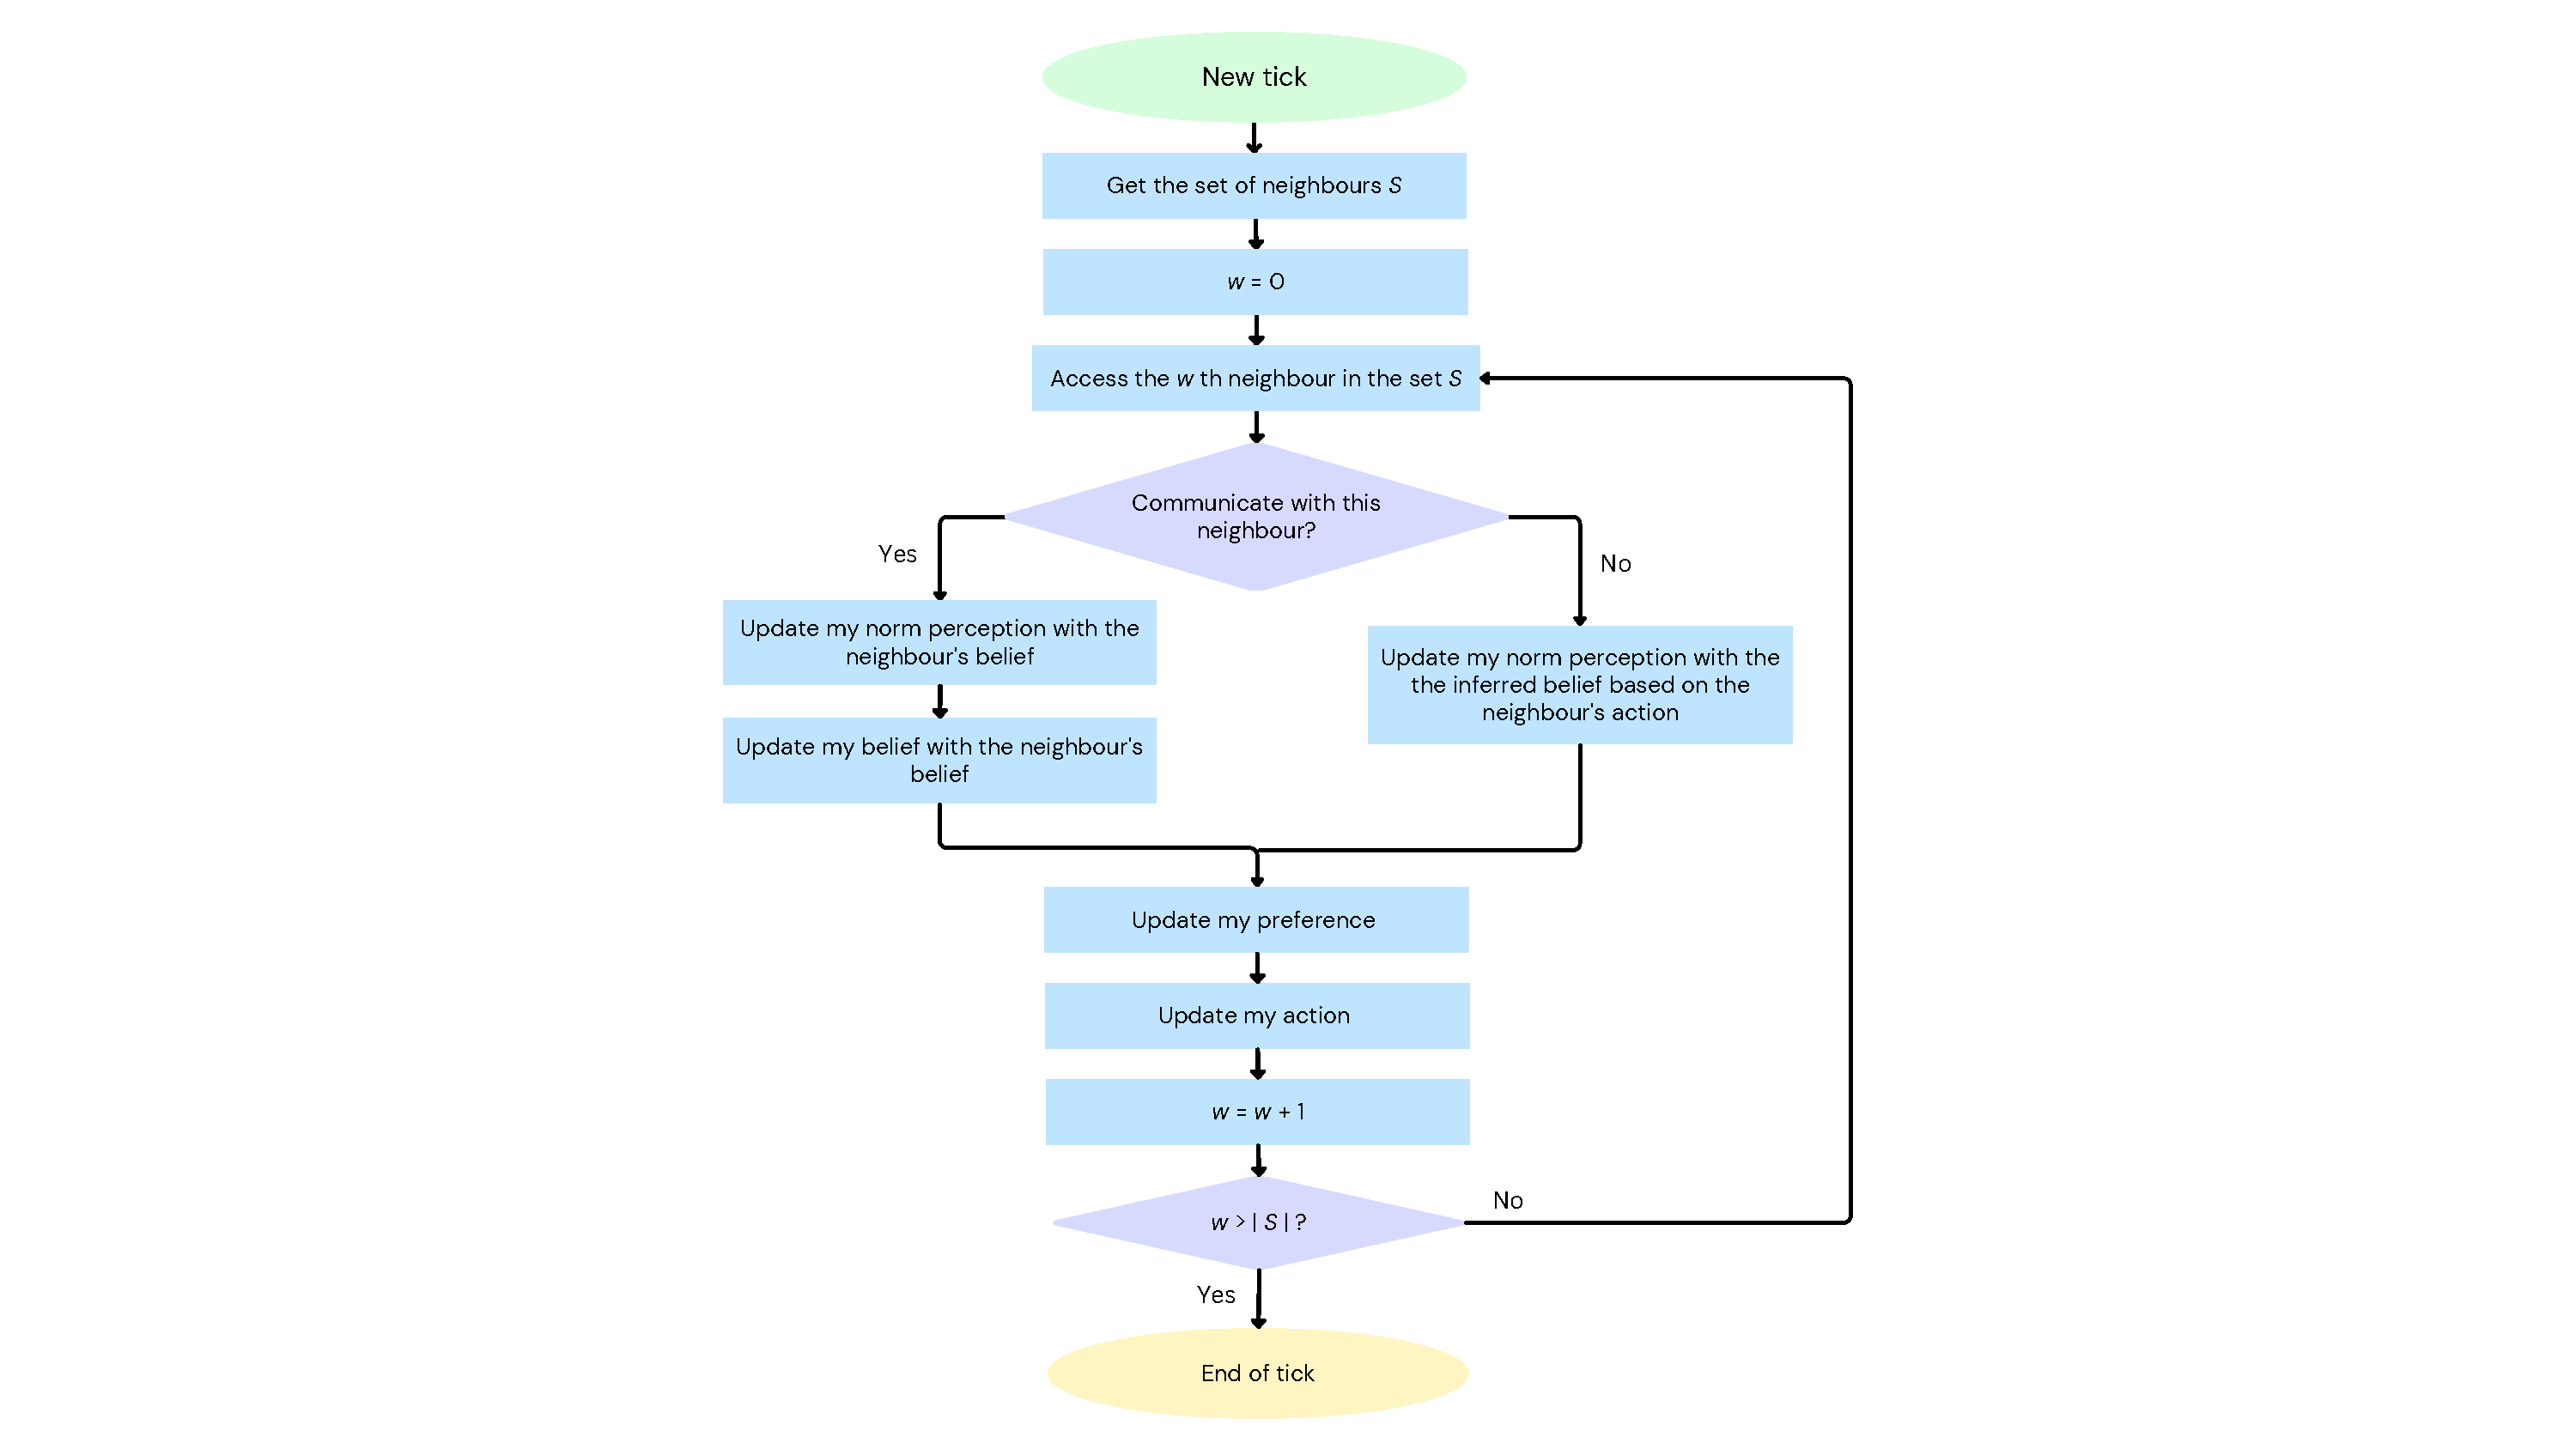
\includegraphics[width=0.8\columnwidth]{./figures/diss_flow_chart.pdf}
  \caption{\textbf{Main updating procedure.} The flow chart shows each agent's behaviour at each time step.}
  \label{fig:1}
\end{figure}

Agent \(i\), upon communicating with and accessing the belief of
neighbour \(j\), updating its own belief with bounded confidence. The
bounded confidence model is able to capture the ubiquitous psychological
phenomenon of being more likely to be influenced by people like
ourselves while keeps the computation simple \textbf{(Cialdini \&
Goldstein, 2004)}. Previous research has successfully nested the bounded
confidence model of opinion dynamics in the framework of the CODA model
in the context of a social network, which serves as a foundation for the
current model \textbf{(Zhan et al., 2022)}. Specifically, agent \(i\)
updates its belief based on neighbour \(j\)'s belief using the following
equation:

\begin{equation}
    B_i^{\prime} = \begin{cases}
        B_i, \;\;\;\;\;\;\;\;\;\;\;\;\;\;\;\;\;\;\;\;\;\;\; \text{if} \: |B_i - B_j| > \epsilon_i \\
        B_i + \alpha (B_j - B_i), \; \text{if} \: |B_i - B_j| \le \epsilon_i
    \end{cases}
\end{equation}

where \(\alpha \in (0,0.5]\) is the convergence parameter and
\(\epsilon_i\) is the bounded confidence threshold of agent \(i\) which
is a value drawn from an exponential distribution with the mean
\(\epsilon_{mean}\) and is a fixed value over time. An exponential
distribution is chosen so that the value is guaranteed to be greater
than zero but does not have an upper limit (The same reason applies to
other parameters that are drawn from an exponential distribution).

Agents update their norm perception \(N_i\) following the Bayesian
inference model \textbf{(Krauß et al.,1999)}. Perception of social norms
is very suitable to be modelled using models of probabilistic inference
such as the Bayesian inference model. This is because norm perception
can be seen as a piece of abstract knowledge that is inferred from
limited observational data, as we can state what we believe to be most
others' beliefs while we are only able to observe (at most) the beliefs
and actions of our acquaintances. To understand this kind of beliefs,
cognitive scientists have been using various probabilistic models for
conceptualisation \textbf{(Tenenbaum et al., 2011; Chater et al.,
2006)}. The present research adopts one specific type of probability
models, the Bayesian inference model, to model norm perception. The
Bayesian model is chosen since it is widely adopted in research of human
perception and memory and has been shown adequate in modelling inference
about everyday events \textbf{(Griffiths and Tenenbaum, 2006; Tavoni et
al., 2022)}.

Using Bayes' theorem, we can update the conditional probability of agent
\(i\)'s norm perception given evidence using the following equation:

\begin{equation}
\label{eq:2}
f(N_i \mid E_i) = \frac{f(N_i) f(E_i \mid N_i)}{\int f(N_i) f(E_i \mid N_i) dN_i},
\end{equation}

where \(f(N_i)\) denotes the prior probability of norm perception of
agent \(i\), \(E_i\) the evidence (either agent \(j\)'s belief or
inferred belief from its action, see Equation \ref{eq:5}), and
\(f(E_i \mid N_i)\) the conditional probability of the evidence given
\(N_i\). Assuming normal distributions for both \(f(N_i)\) and
\(f(E_i \mid N_i)\), the following updating rules for the mean and
standard deviation of agents' norm perception can be derived (see the
appendices for the derivation):

\begin{equation}
\label{eq:3}
\mu_{N_i}^{\prime} = \lambda \mu_{N_i} + (1 - \lambda) E_i,
\end{equation}

\begin{equation}
\label{eq:4}
\sigma_{N_i}^{\prime2} = \lambda \sigma_{N_i}^2,
\end{equation}

where \(\lambda = \frac{c_i^2}{c_i^2 + \sigma_{N_i}^2}\). The variable
\(c_i\) is the degree of agent \(i\)'s lack of confidence in its norm
perception (i.e., the standard deviation of the conditional probability
of the evidence, \(f(E_i \mid N_i)\)). \(c_i\) is a value drawn from an
exponential distribution with the mean \(c_{mean}\) and is a fixed value
over time.

Since agents may or may not communicate with neighbour \(j\), the value
of \(E\) is given by the following equation:

\begin{equation}
\label{eq:5}
  E_i = \begin{cases}
    B_j, \;\;\;\;\;\;\;\;\;\;\;\;\;\;\; \text{if agent} \; i \; \text{communicates with agent} \; j \\
    P(B_j \mid A_j), \;\; \text{if agent} \; i \; \text{doesn't communicate with agent} \; j
  \end{cases}
\end{equation}

\(P(B_j \mid A_j = 1) = 0.9\) and \(P(B_j \mid A_j = 0) = 0.1\) by
stipulation in the simulations reported in the present research.

After updating their belief and norm perception, agents update
preference and action regarding WWOH based on these two values. The
preference is determined by the equation

\begin{equation}
  P_i = r_i B_i + (1 - r_i) N_i,
\end{equation}

where \(r_i\) represents each agent's resistance to social norm, which
is drawn from an exponential distribution with the mean \(r_{mean}\) and
is a fixed value over time. The WWOH action is determined by the
equation:

\begin{equation}
  A_i = \begin{cases}
    0, \;\; \text{if} \; P_i \in [0, 0.5)\\
    1, \;\; \text{if} \; P_i \in [0.5, 1]
  \end{cases}
\end{equation}

\hypertarget{interventions}{%
\subsubsection{Interventions}\label{interventions}}

A social norm intervention using summary information about the norm is
implemented in the model. In the intervention, the summary information
about the true norm \(T_t = \overline{B_i}\) is distributed to all
agents at the selected time step \(t\). Agents take this as a persuasive
message, the credibility of which is perceived as \(s_i\), and update
their norm perception in a similar manner as they update their beliefs
about WWOH upon learning other agents' beliefs. Formally, this is
expressed as:

\begin{equation}
  \mu_{N_i}^{\prime} = \begin{cases}
    \mu_{N_i}, \;\;\;\;\;\;\;\;\;\;\;\;\;\;\;\;\;\;\;\;\;\;\;\;\;\;\;\;\;\;\;\; \text{if} \: |\mu_{N_i} - T_t| > \epsilon_i \\
    \mu_{N_i} + \alpha \cdot s_i \cdot (T_t - \mu_{N_i}), \; \text{if} \: |\mu_{N_i} - T_t| \le \epsilon_i
  \end{cases}
\end{equation}

The variable \(s_i\) is drawn from a truncated normal distribution
(between 0 and 1) with the mean \(s_{mean}\) and \(s_{sd}\) and is a
fixed value over time.

The time steps when the intervention is implemented are \(t_1 = 30\),
\(t_2 = 40\), and \(t_3 = 50\). The intervention is implemented in three
ways. First, the summary information is distributed once at time
\(t_1\). Second, the information is distributed twice at time \(t_1\)
and \(t_2\). Finally, the information is distributed at all three time
steps. At the intervention time steps, agents do not update their norm
perception in the regular manner via observation (or communication) but
only through the summary information. Other procedures remain unchanged.

\hypertarget{simulations}{%
\subsection{Simulations}\label{simulations}}

The model will be run using the parameter values listed in Table
\ref{tab:parameters}. For each set of parameter combination, 25
simulations will be run and each simulation will run for 150 time steps.
The model is written and the simulations are run in NetLogo 6.3
\textbf{(Wilensky, 1999)}. The model and data are available in the
online repository (OSF: \textbf{(insert link here)}).

The following main outcomes are measured at each time step of the
simulations: 1) \(P_U = P(\mu_{N_i} < P_s)\), proportion of agents who
underestimate the proportion of WWOH supporters (also referred to as the
rate of underestimation), 2)
\(P_I = P((B_i \ge 0.5 \wedge A_i = 0) \vee (B_i < 0.5 \wedge A_i = 1))\),
the proportion of agents with inconsistent beliefs and actions regarding
WWOH (also referred to as the rate of inconsistency), and 3)
\(P_A = P(A_i = 1)\), proportion of agents who demonstrate WWOH actions
(also referred to the rate of WWOH actions). Outcome 1) and 2) are the
key measures for PI regarding WWOH, despite assuming different
definitions of PI. Outcome 1) follows the empirical study about Saudi
Arabia and defines PI as the phenomenon that exists if and only if more
than half of all agents underestimate the true proportion of agents who
support WWOH \textbf{(Bursztyn et al., 2020)}. Outcome 2) follows
previous models of PI and defines PI as the phenomenon that exists if
and only if more than half of all agents act differently from their
private beliefs \textbf{(e.g., Ye et al., 2019)}.

For exploratory and potentially explanatory purpose, four extra outcomes
are also measured at each time step: 1) \(\overline{B_i}\), average
beliefs regarding WWOH among all agents, 2) \(P_s = P(B_i \ge 0.5)\),
proportion of agents who are WWOH supporters, 3)
\(\overline{\mu_{N_i}}\), average norm perception regarding WWOH among
all agents, and 4) \(\overline{\sigma_{N_i}}\), average uncertainty of
norm perception among all agents.

\newpage

\begin{landscape}

\begingroup
\renewcommand{\arraystretch}{1.5}

\begin{table}[ht]
  \centering
  \caption{\textbf{A List of Parameters}}
  \label{tab:parameters}
  \resizebox{\columnwidth}{!}{
  \begin{tabular}{>{\centering\arraybackslash}p{0.2\textwidth}>{\centering\arraybackslash}p{0.6\textwidth}>{\centering\arraybackslash}p{0.2\textwidth}}
    \toprule
    \textbf{Parameters} & \textbf{Description} & \textbf{Values} \\
    \midrule
    \multicolumn{3}{l}{\textit{Model setup}} \\
    $n$ & \multicolumn{1}{l}{Number of agents} & 100 \\
    $p_r$ & \multicolumn{1}{l}{Rewiring probability in small-world network setup} & 0.3, 0.5, 0.7 \\
    $p_s$ & \multicolumn{1}{l}{Proportion of agents who are WWOH supporters at the beginning of simulations} & 0.8 \\
    $\mu_B$ & \multicolumn{1}{l}{Mean of the normal distribution from which the initial belief regarding WWOH is drawn} & 0.5 \\
    $\sigma_B$ & \multicolumn{1}{l}{Standard deviation of the above distribution} & 0.2 \\
    $\mu_{N_{prior}}$ & \multicolumn{1}{l}{Mean of the normal distribution from which the initial norm perception is drawn} & 0.5 \\
    $\sigma_{N_{prior}}$ & \multicolumn{1}{l}{Standard deviation of the above distribution} & 0.2 \\
    $p_A$ & \multicolumn{1}{l}{Proportion of agents who demonstrate WWOH action at the beginning of simulations} & 0.05 \\
    \multicolumn{3}{l}{\textit{Updating Procedures}} \\
    $p_c$ & \multicolumn{1}{l}{Probability of communication with each neighbour} & 0.1, 0.3, 0.5 \\
    $\epsilon_{mean}$ & \multicolumn{1}{l}{Mean of the exponential distribution from which the bounded confidence threshold is drawn} & 0.3, 0.5, 0.7 \\
    $\alpha$ & \multicolumn{1}{l}{Convergence parameter} & 0.1, 0.3, 0.5 \\
    $c_{mean}$ & \multicolumn{1}{l}{Mean of the exponential distribution from which the agents' degree of lack of confidence in norm perception is drawn} & 0.1, 0.3, 0.5 \\
    $r_{mean}$ & \multicolumn{1}{l}{Mean of the exponential distribution from which the resistance to norm is drawn} & 0.1, 0.3, 0.5 \\
    \multicolumn{3}{l}{\textit{Interventions}} \\
    $s_{mean}$ & \multicolumn{1}{l}{Mean of the normal distribution from which the credibility perception of the summary information is drawn} & 0.3, 0.5, 0.7 \\
    $s_{sd}$ & \multicolumn{1}{l}{Standard deviation of the above distribution} & 0.2 \\
    \bottomrule
  \end{tabular}}

\end{table}

\endgroup

\end{landscape}

\newpage

\hypertarget{results-2000-2500}{%
\section{Results (2000-2500)}\label{results-2000-2500}}

Given the large number of varying parameters and resulting parameter
combinations, not all results are reported in the main text for the sake
of brevity. The results that support the claims in this section but
can't be reported here due to space limitation are reported in the
Appendices.

\hypertarget{factors-associated-with-persistent-pluralistic-ignorance}{%
\subsection{Factors Associated With Persistent Pluralistic
Ignorance}\label{factors-associated-with-persistent-pluralistic-ignorance}}

To explore the factors associated with the persistent level of
pluralistic ignorance regarding WWOH that was found in the empirical
study, the present study investigates the three outcome variables when
no intervention is implemented. Linear regressions with full
interactions are run including all varied parameters as predictors
(except for \(s_{mean}\)). Table \ref{tab:2} shows the effects of each
parameter at the final time step on the rate of underestimation, the
rate of inconsistency, and the rate of WWOH actions when controlled for
other parameters. All else equal, no parameters or interaction terms
have statistically significant effects on the rate of underestimation.
The probability of communication with neighbours (\(p_c\)) and mean
resistance to norm (\(r_{mean}\)) have negative effects on the rate of
inconsistency and positive effects on the rate of WWOH actions. No
interaction term has a significant effect on either the rate of
inconsistency or the rate of WWOH actions.

\begin{figure}[h]
  \centering
  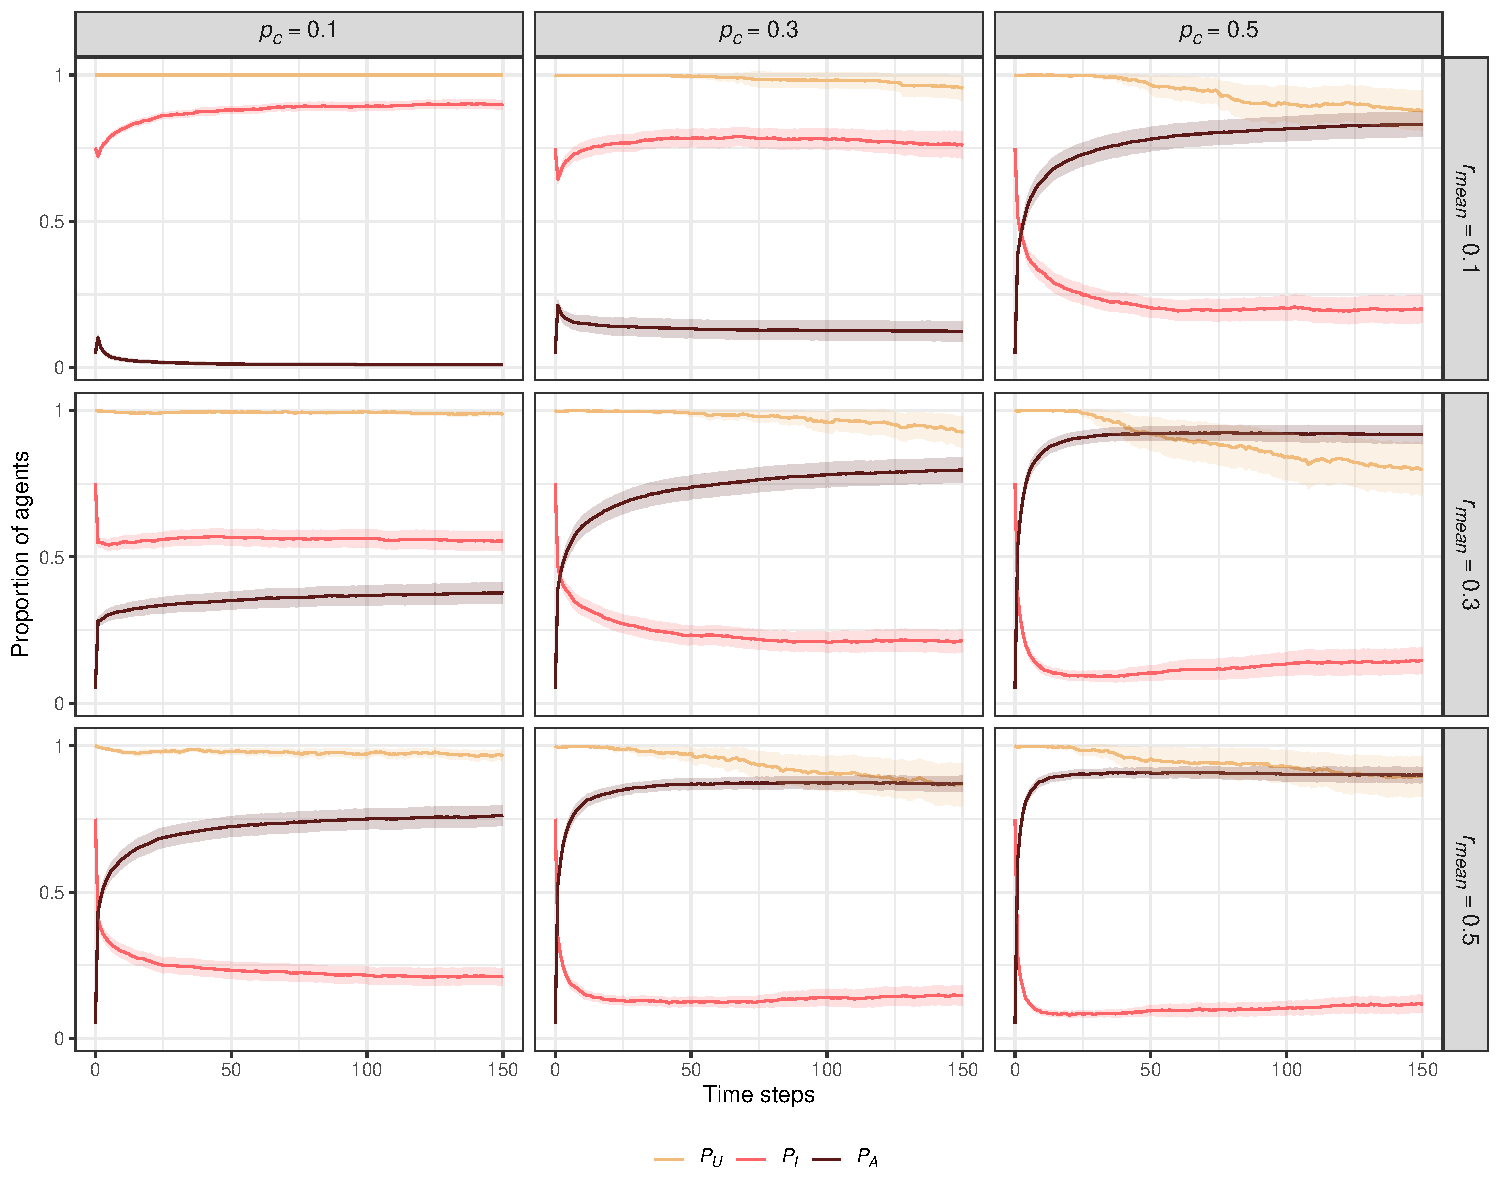
\includegraphics[width=1\columnwidth]{./figures/factor_for_pi.pdf}
  \caption{\textbf{Pluralistic ignorance and WWOH action over time when no intervention is implemented.} $P_U$, $P_I$, $P_A$ denote the rate of underestimation, the rate of inconsistency, and the rate of WWOH actions, respectively. Central lines are average values of simulations with the same parameter setting, and shaded areas are the 95\% confidence intervals. Probability of communication with neighbours $p_c$ is shown on facet columns, and the mean resistance to norm $r_{mean}$ is shown on facet rows. Parameters not shown on the plot are set at the following values: $p_r = 0.5$, $\epsilon_{mean} = 0.5$, $\alpha = 0.3$, $c_{mean} = 0.3$.}
  \label{fig:2}
\end{figure}

To revealed the process of the two parameters influencing the outcomes,
full processes of the simulations are plotted. As Figure \ref{fig:2}
shows, both the probability of communication and mean resistance to norm
influence the change of outcome variables over time. Particularly,
resistance to norm being equal, higher probability of communication
decreases the rate of underestimation and the rate of inconsistency
while increasing the rate of WWOH actions. Higher resistance to norm has
similar effects on the three outcome variables when the probability of
communication is held equal.

\begingroup
\renewcommand{\arraystretch}{1.5}

\begin{table}
\caption{\textbf{Effects of parameters on pluralistic ignorance and WWOH action at the final time step when no intervention is implemented}}
\centering
\begin{threeparttable}
\resizebox{\linewidth}{!}{
\begin{tabular}[t]{>{\raggedright\arraybackslash}p{0.5in}cccccccccccc}
\toprule
\multicolumn{1}{c}{ } & \multicolumn{4}{c}{$P_U$} & \multicolumn{4}{c}{$P_I$} & \multicolumn{4}{c}{$P_A$} \\
\cmidrule(l{3pt}r{3pt}){2-5} \cmidrule(l{3pt}r{3pt}){6-9} \cmidrule(l{3pt}r{3pt}){10-13}
\multicolumn{1}{c}{\em{ }} & \multicolumn{1}{c}{$\beta$} & \multicolumn{1}{c}{\em{se}} & \multicolumn{1}{c}{\em{t}} & \multicolumn{1}{c}{\em{p}} & \multicolumn{1}{c}{$\beta$} & \multicolumn{1}{c}{\em{se}} & \multicolumn{1}{c}{\em{t}} & \multicolumn{1}{c}{\em{p}} & \multicolumn{1}{c}{$\beta$} & \multicolumn{1}{c}{\em{se}} & \multicolumn{1}{c}{\em{t}} & \multicolumn{1}{c}{\em{p}}\\
\midrule
$p_r$ & 0.03 & 0.32 & 0.10 & .919 & 0.21 & 0.27 & 0.76 & .447 & –0.23 & 0.27 & –0.84 & .402\\
$p_c$ & 0.34 & 0.49 & 0.69 & 0.492 & \textbf{–1.65} & 0.42 & –3.97 & <.001 & \textbf{1.93} & 0.42 & 4.59 & <.001\\
$\epsilon_{mean}$ & 0.16 & 0.32 & 0.50 & 0.616 & 0.31 & 0.27 & 1.13 & .259 & –0.13 & 0.27 & –0.47 & .638\\
$\alpha$ & 0.30 & 0.49 & 0.60 & 0.546 & 0.28 & 0.42 & 0.68 & .495 & –0.13 & 0.42 & –0.32 & .749\\
$c_{mean}$ & 0.09 & 0.49 & 0.17 & 0.861 & –0.23 & 0.42 & –0.54 & .588 & 0.32 & 0.42 & 0.77 & .441\\
$r_{mean}$ & –0.17 & 0.49 & –0.34 & 0.736 & \textbf{–1.58} & 0.42 & –3.80 & <.001 & \textbf{1.88} & 0.42 & 4.48 & <.001\\
\bottomrule
\end{tabular}}
\begin{tablenotes}
\small
\item \textit{Note.} $P_U$, $P_I$, $P_A$ denote the rate of underestimation, the rate of inconsistency, and the rate of WWOH \\actions, respectively. Linear regressions are run with full interaction. Intercepts and interaction terms \\are omitted for brevity (see the Appendices for the full table). Statistically significant coefficients are in \\ bold.
\end{tablenotes}
\end{threeparttable}
\label{tab:2}
\end{table}

\endgroup

When the resistance to norm is low (\(r_{mean} = 0.1\), facet row one),
low (\(p_c = 0.1\)) and medium probability of communication
(\(p_c = 0.3\)) keep the rate of underestimation and the rate of
inconsistency above \(0.5\), and the rate of WWOH actions low.
Pluralistic ignorance exists by either one of the two definitions
(\(P_U > 0.5\) or \(P_I > 0.5\)). When the resistance to norm is low and
the probability of communication is high (\(p_c = 0.5\)), the rate of
underestimation slightly decreases but still remains above \(0.5\),
while the rate of inconsistency drops under \(0.5\) and the rate of WWOH
increases drastically to a high level.

Under the condition of medium resistance to norm (\(r_{mean} = 0.3\),
facet row 2) and low probability of communication (\(p_c = 0.1\)), the
rate of underestimation remains virtually constant around \(1\). The
rate of inconsistency decreases moderately but still remains above
\(0.5\), and the rate of WWOH actions increases moderately. Pluralistic
ignorance also exists by either one of the two definitions. In all other
conditions, although the rate of underestimation remains high, the rate
of inconsistency drops under \(0.5\) and the rate of WWOH increases
quickly at the very beginning of the simulations.

Sensitivity analyses were conducted on other combinations of rewiring
probability (\(p_r\)), bounded confidence threshold
(\(\epsilon_{mean}\)), convergence parameter (\(\alpha\)), and mean lack
of confidence (\(c_{mean}\)), and no qualitative difference in the
results is found (see the Appendices).

\hypertarget{intervention-effects-on-pluralistic-ignorance-and-wwoh-action}{%
\subsection{Intervention Effects on Pluralistic Ignorance and WWOH
Action}\label{intervention-effects-on-pluralistic-ignorance-and-wwoh-action}}

To investigate the the effects of interventions on PI regarding WWOH,
parameter combinations that sustain PI and WWOH action at the level
reported in the empirical study are first identified. The empirical rate
of underestimation of WWOH norm among Saudi men is around \(P_U = 0.8\)
and the rate of WWOH actions is around \(P_A = 0.05\) \textbf{(Bursztyn
et al., 2020)}. One-sample \emph{t}-tests on the outcome variables
reveal that no parameter combinations produce \(P_U\) and \(P_A\) close
to these values (i.e., the empirical rate falls within the 95\%
confidence intervals of \(P_U\) and \(P_A\) produced by the model)
simultaneously at the final time step. Some parameter combinations do
give rise to \(P_U\) close to 0.8, but the rates of WWOH actions are
significantly different from 0.05 (most are over 0.5, see Appendix Table
C1). Some parameter combinations give rise to \(P_A\) close to 0.05.
Although the rates of underestimation under these conditions are also
significantly different from 0.8, most of them lie within a reasonable
proximity to the empirical level (see Appendix Table C1). Therefore, the
parameter combinations that give rise to \(P_A\) close to 0.05 are used
for further analyses.

Linear regressions are run on the rate of underestimation, the rate of
inconsistency, and the rate of WWOH actions using the following model
\footnote{Subscripts are omitted for readability. $c_{mean}$ and $r_{mean}$ are not included as predictors since the former is perfectly correlated with $p_c$ and the latter lacks variation in the data.}:

\begin{equation}
  \begin{aligned}
  y &= a + b_1I + b_2p_r + b_3p_c + b_4\epsilon_{mean} + b_5\alpha + b_6s_{mean} +\\
  &+ b_7I \cdot p_r + b_{8}I \cdot p_c + b_{9}I \cdot \epsilon_{mean} + b_{10}I \cdot \alpha + b_{11}I \cdot s_{mean} + \gamma,
  \end{aligned}
\end{equation}

where \(\gamma\) denotes random errors. Interaction terms are included
to detect potential dependency of the intervention effect on other
parameter values.

The results reveal that all else equal, the intervention does not have a
statistically significant effect on the rate of underestimation, be it
implemented once, twice, or three times. The intervention does have a
significant effect on the rate of inconsistency regardless of the times
for which it is implemented, and its effect depends on \(p_c\),
\(\epsilon_{mean}\), \(\alpha\), and \(s_{mean}\). The intervention has
a significant effect on the rate of WWOH actions only when it is
implemented twice or three times, and this effect also depends on
\(p_c\), \(\epsilon_{mean}\), \(\alpha\), and \(s_{mean}\) (see Appendix
Table C2 for the full model results).

To show the above results more clearly, the effects of the intervention
under different combinations of parameter values are plotted (Figure
\ref{fig:3} and \ref{fig:4}). As Figure \ref{fig:3} shows, the
decreasing effect of the intervention on the rate of inconsistency
increases with the the probability of communication (\(p_c\)), mean
perceived credibility (\(s_{mean}\)), convergence parameter
(\(\alpha\)), and mean bounded confidence threshold
(\(\epsilon_{mean}\)). The decreasing effect also increases with the
number of times the intervention is implemented, and the increase is
especially pronounced when the times increase from twice to three times.
When the intervention is implemented once, its effect remains close to 0
under all parameter combinations.

\begin{figure}[h]
  \centering
  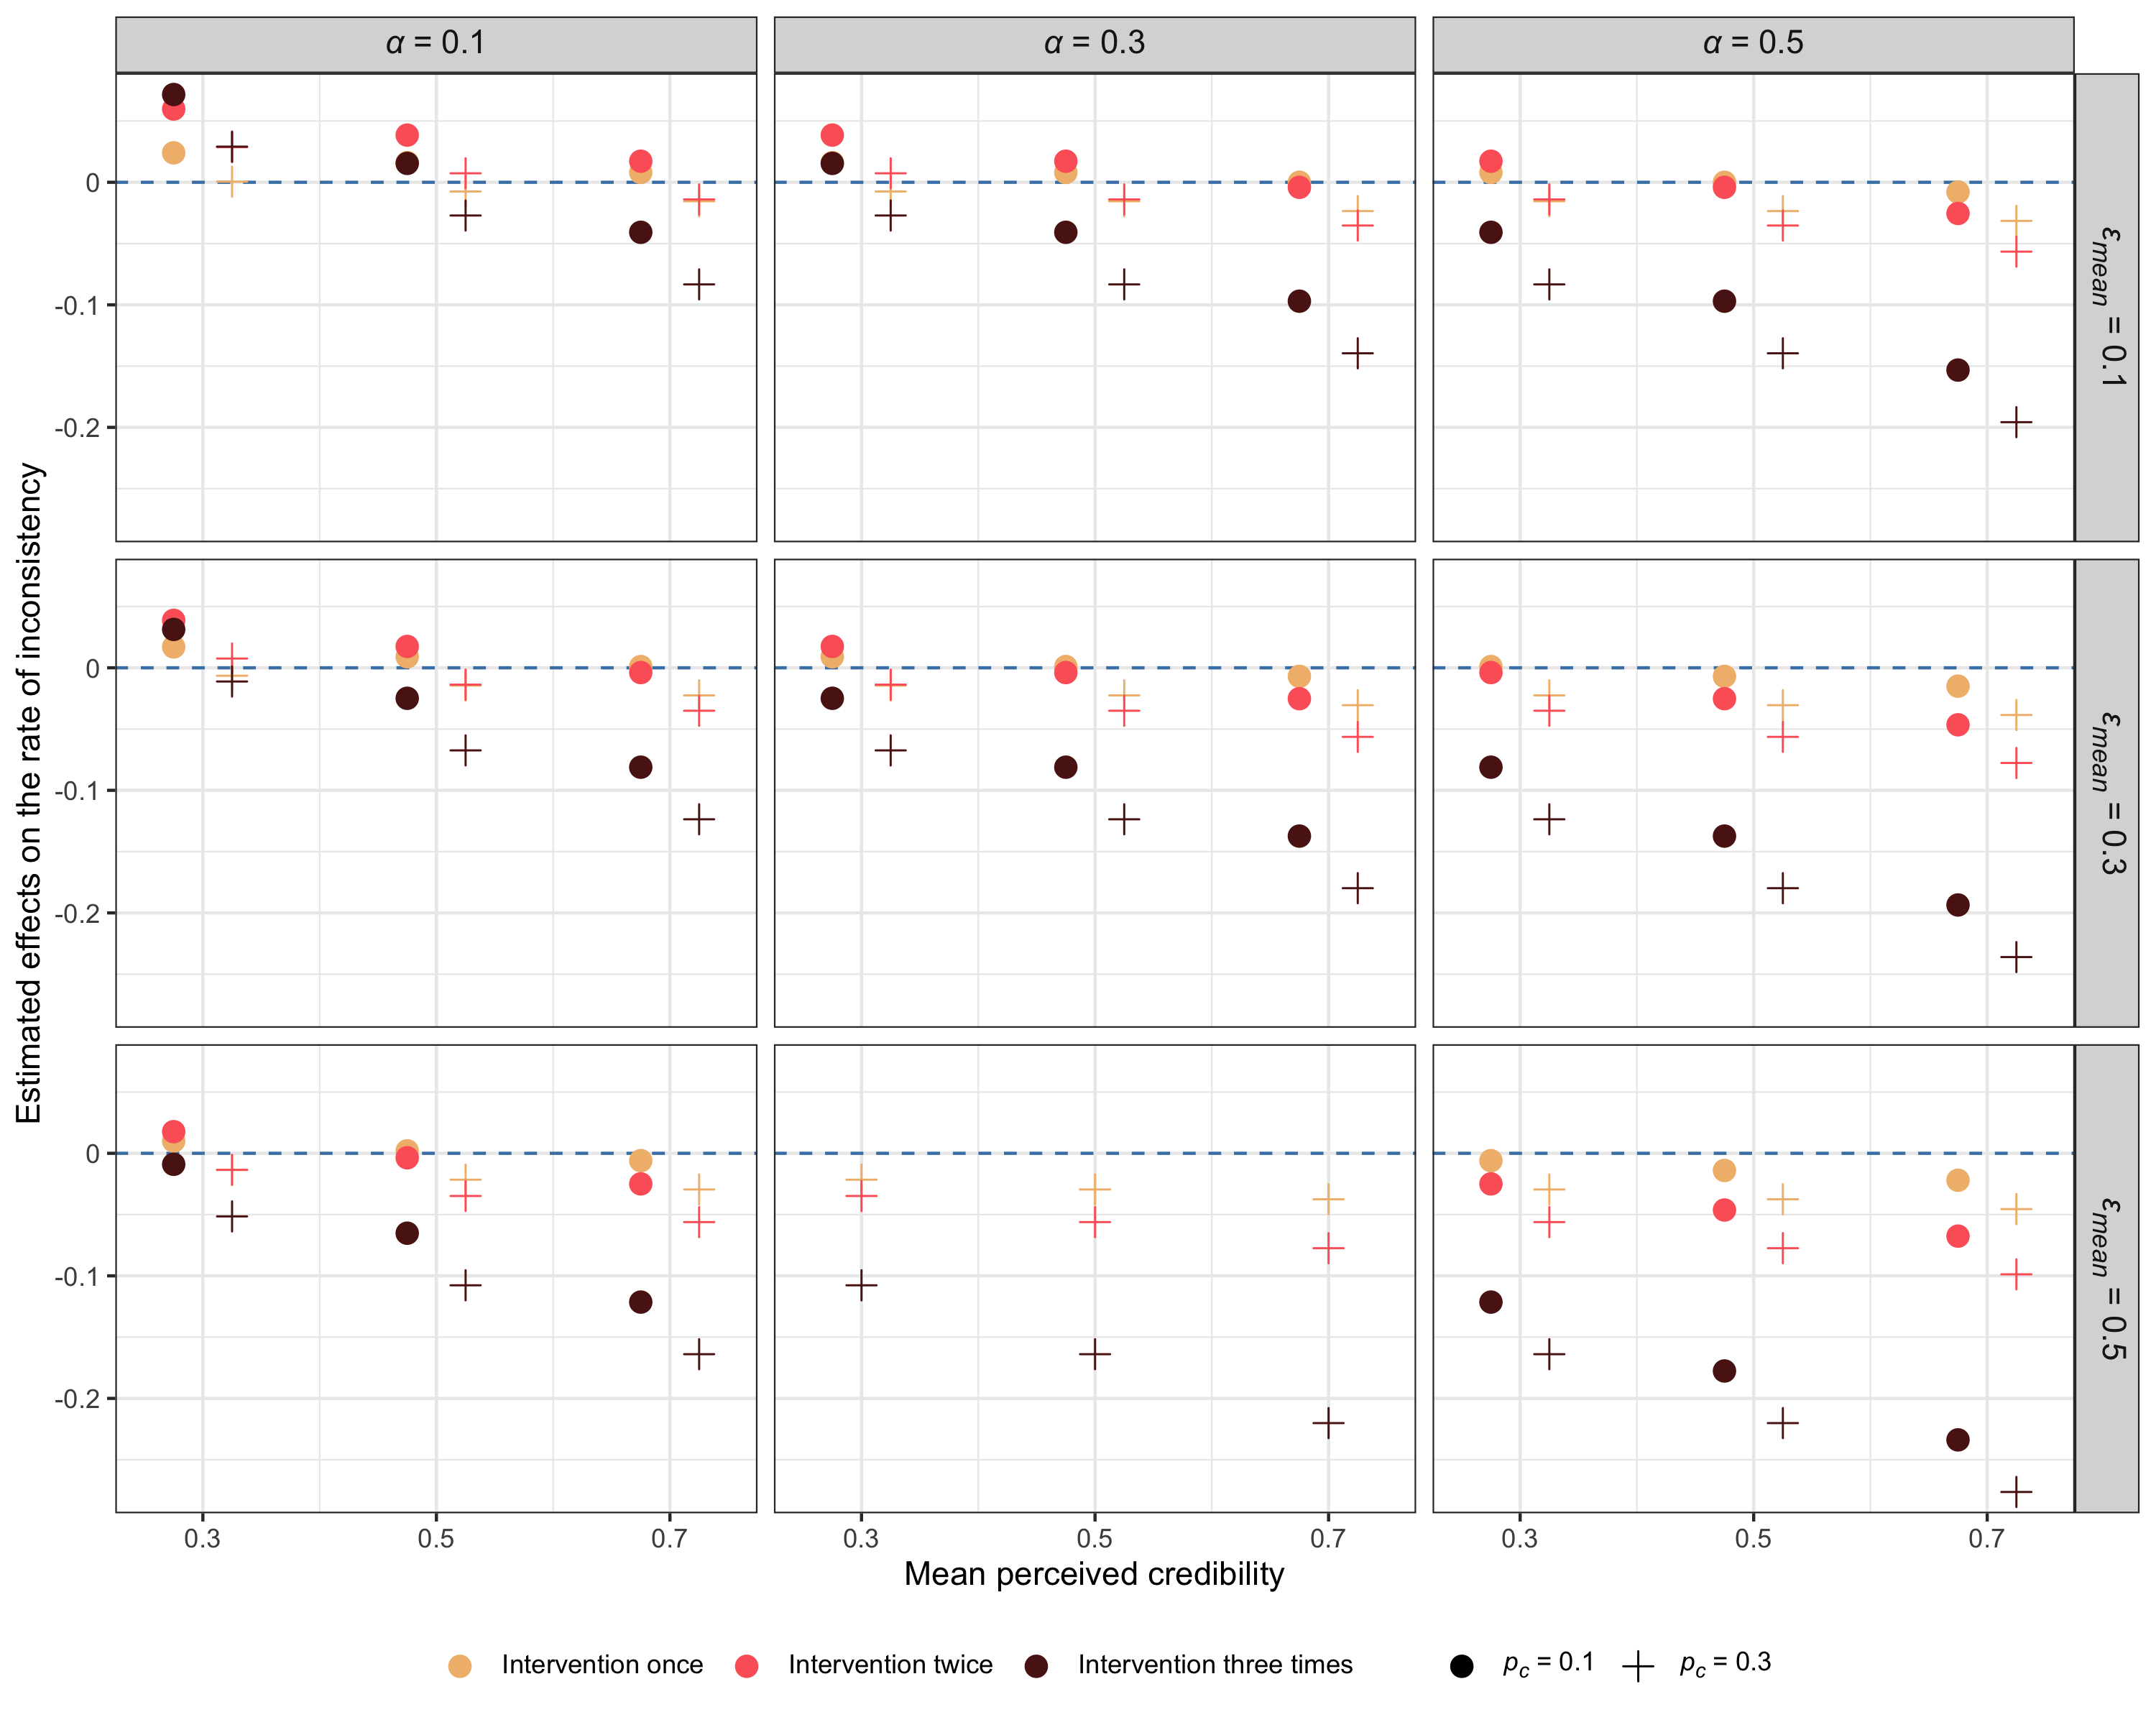
\includegraphics[width=1\columnwidth]{./figures/intervention_effect_p_inconsistency.png}
  \caption{\textbf{Estimated effects of the intervention on the rate of inconsistency at the final time step.} Point estimates of the effects of the intervention are plotted under different combinations of parameter values. The blue dashed line indicates 0 effect. Convergence parameter $\alpha$ is shown on facet columns, and the mean bounded confidence threshold $\epsilon_{mean}$ is shown on facet rows. Parameters not shown on the plot are set at the following value: $p_r = 0.5$.}
  \label{fig:3}
\end{figure}

Likewise, the increasing effect of the intervention on the rate of WWOH
actions increases with the the probability of communication (\(p_c\)),
mean perceived credibility (\(s_{mean}\)), convergence parameter
(\(\alpha\)), and mean bounded confidence threshold
(\(\epsilon_{mean}\)) (Figure \ref{fig:4}). The increasing effect also
increases with the number of times the intervention is implemented. When
the intervention is implemented once, its effect remains close to 0
under all parameter combinations.

\begin{figure}[h]
  \centering
  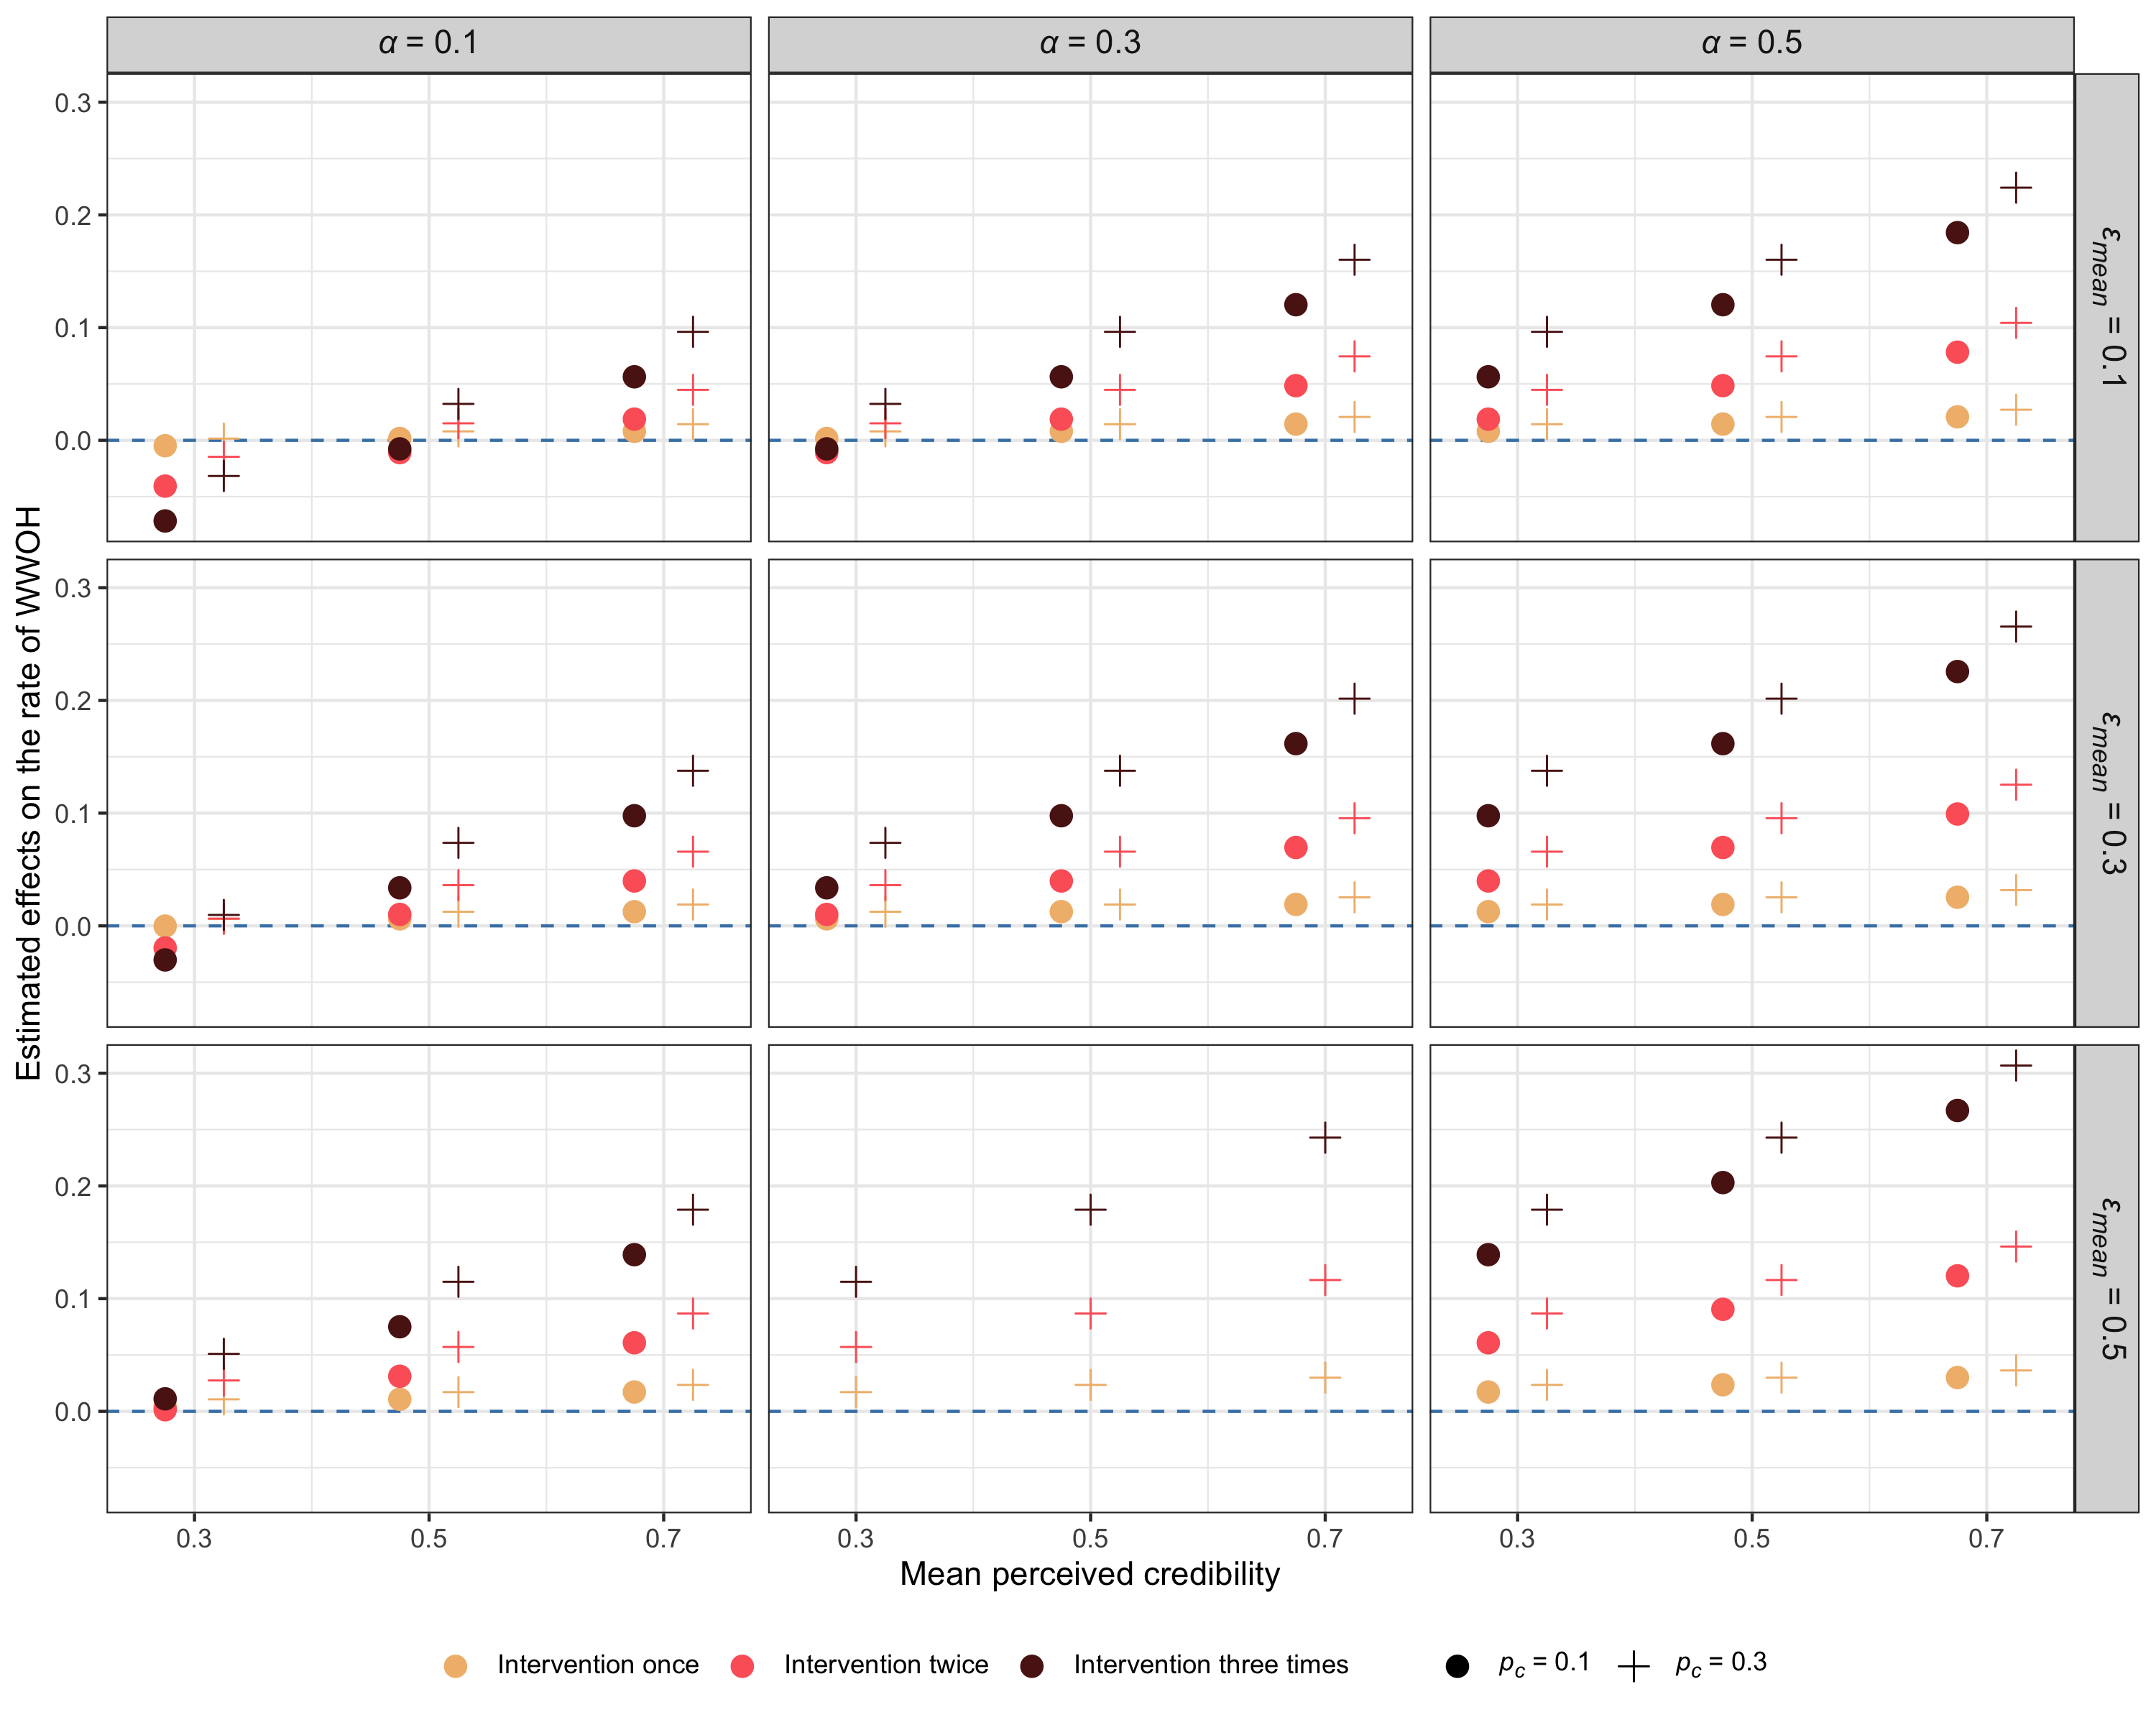
\includegraphics[width=1\columnwidth]{./figures/intervention_effect_p_wwoh.png}
  \caption{\textbf{Estimated effects of the intervention on the rate of WWOH actions at the final time step.} Point estimates of the effects of the intervention are plotted under different combinations of parameter values. The blue dashed line indicates 0 effect. Convergence parameter $\alpha$ is shown on facet columns, and the mean bounded confidence threshold $\epsilon_{mean}$ is shown on facet rows. Parameters not shown on the plot are set at the following value: $p_r = 0.5$.}
  \label{fig:4}
\end{figure}

\hypertarget{discussion-and-conclusion-1000-1500}{%
\section{Discussion and Conclusion
(1000-1500)}\label{discussion-and-conclusion-1000-1500}}

\newpage

\hypertarget{reference}{%
\section*{Reference}\label{reference}}
\addcontentsline{toc}{section}{Reference}

\newpage

\hypertarget{appendices}{%
\section*{Appendices}\label{appendices}}
\addcontentsline{toc}{section}{Appendices}

\hypertarget{appendix-a-the-derivation-of-equation-3-and-4}{%
\subsection*{Appendix A: The Derivation of Equation 3 and
4}\label{appendix-a-the-derivation-of-equation-3-and-4}}
\addcontentsline{toc}{subsection}{Appendix A: The Derivation of Equation
3 and 4}

Since agents' norm perception \(N_i\) is a random variable with a normal
distribution with the mean \(\mu_{N_i}\) and standard deviation
\(\sigma_{N_i}\), we have the probability density function (PDF) of
\(N_i\) as:

\begin{equation*}
f(N_i) \propto \text{exp}(-\frac{(N_i - \mu_{N_i})^2}{2\sigma_{N_i}^2}).
\end{equation*}

The conditional PDF of the evidence given agent \(i\)'s prior norm
perception in Equation \ref{eq:2} is given by

\begin{equation*}
f(E_i \mid N_i) \propto \text{exp}(-\frac{(E_i - N_i)^2}{2c_i^2}).
\end{equation*}

Following the Equation \ref{eq:2}, we have the posterior PDF of agent
\(i\)'s norm perception as

\begin{equation*}
  \begin{aligned}
    f(N_i \mid E_i) &= C \cdot \text{exp}(-\frac{(N_i - \mu_{N_i})^2}{2\sigma_{N_i}^2}) \text{exp}(- \frac{(E_i - N_i)^2}{2c_i^2})\\
      &= C \cdot \text{exp}(-\frac{(N_i - \mu_{N_i})^2}{2\sigma_{N_i}^2} - \frac{(E_i - N_i)^2}{2c_i^2})\\
      &= C \cdot \text{exp}(- \frac{(N_i - \mu_{N_i}^{\prime})^2}{2\sigma_{N_i}^{\prime2}} - \frac{(E_i - \mu_{N_i})^2}{2(\sigma_{N_i}^2 + c_i^2)}),
  \end{aligned}
\end{equation*}

where \(C\) is a normalising constant. Since the second term in the
exponent does not involve the random variable \(N_i\), we can
incorporate it into the constant and rewrite the expression as

\begin{equation*}
  f(N_i \mid E_i) \propto \text{exp}(- \frac{(N_i - \mu_{N_i}^{\prime})^2}{2\sigma_{N_i}^{\prime2}}),
\end{equation*}

where

\begin{equation*}
  \mu_{N_i}^{\prime} = \frac{E_i \sigma_{N_i}^2 + \mu_{N_i} c_i^2}{\sigma_{N_i}^2 + c_i^2} \;\; \text{and} \;\; \sigma_{N_i}^{\prime2} = \frac{\sigma_{N_i}^2 c_i^2}{\sigma_{N_i}^2 + c_i^2}.
\end{equation*}

Substituting \(\frac{c_i^2}{c_i^2 + \sigma_{N_i}^2}\) with \(\lambda\)
gives the equations in the main text.

\hypertarget{appendix-b-supplementary-results-on-the-factors-associated-with-persistent-pi}{%
\subsection{Appendix B: Supplementary Results on the Factors Associated
with Persistent
PI}\label{appendix-b-supplementary-results-on-the-factors-associated-with-persistent-pi}}

\textbf{table: full regression model}

\textbf{sensitivity analysis on the effect of p\_com and r\_mean}

\begin{landscape}

\hypertarget{appendix-c-effects-of-interventions-on-pluralistic-ignorance-and-wwoh-action}{%
\subsection{Appendix C: Effects of Interventions on Pluralistic
Ignorance and WWOH
Action}\label{appendix-c-effects-of-interventions-on-pluralistic-ignorance-and-wwoh-action}}

\renewcommand{\thetable}{C1}

\begin{ThreePartTable}
\begin{TableNotes}
\small
\item \textit{Note.} $P_U$ and $P_A$ denote the rate of underestimation and the rate of WWOH actions, respectively. The values of $P_U$ are tested against the null hypothesis $P_U = 0.8$, and the values of $P_A$ are tested against the null hypothesis $P_A = 0.05$. The \textit{p} values are adjusted for multiple comparison using the methods of Benjamini, Hochberg, and Yekutieli.
\end{TableNotes}
\begin{longtable}[t]{cccccccccccccc}
\caption{\textbf{Parameter combinations that sustain PI at the empirical level}}\\
\toprule
\multicolumn{6}{c}{ } & \multicolumn{4}{c}{$P_U$} & \multicolumn{4}{c}{$P_A$} \\
\cmidrule(l{3pt}r{3pt}){7-10} \cmidrule(l{3pt}r{3pt}){11-14}
\multicolumn{1}{c}{$p_r$} & \multicolumn{1}{c}{$p_c$} & \multicolumn{1}{c}{$\epsilon_{mean}$} & \multicolumn{1}{c}{$\alpha$} & \multicolumn{1}{c}{$c_{mean}$} & \multicolumn{1}{c}{$r_{mean}$} & \multicolumn{1}{c}{\em{M}} & \multicolumn{1}{c}{\em{SD}} & \multicolumn{1}{c}{95\%CI [LL, UL]} & \multicolumn{1}{c}{\em{p}} & \multicolumn{1}{c}{\em{M}} & \multicolumn{1}{c}{\em{SD}} & \multicolumn{1}{c}{95\%CI [LL, UL]} & \multicolumn{1}{c}{\em{p}}\\
\midrule
\endfirsthead
\caption[]{\textbf{Parameter combinations that sustain PI at the empirical level} \textit{(continued)}}\\
\toprule
\multicolumn{6}{c}{ } & \multicolumn{4}{c}{$P_U$} & \multicolumn{4}{c}{$P_A$} \\
\cmidrule(l{3pt}r{3pt}){7-10} \cmidrule(l{3pt}r{3pt}){11-14}
\multicolumn{1}{c}{$p_r$} & \multicolumn{1}{c}{$p_c$} & \multicolumn{1}{c}{$\epsilon_{mean}$} & \multicolumn{1}{c}{$\alpha$} & \multicolumn{1}{c}{$c_{mean}$} & \multicolumn{1}{c}{$r_{mean}$} & \multicolumn{1}{c}{\em{M}} & \multicolumn{1}{c}{\em{SD}} & \multicolumn{1}{c}{95\%CI [LL, UL]} & \multicolumn{1}{c}{\em{p}} & \multicolumn{1}{c}{\em{M}} & \multicolumn{1}{c}{\em{SD}} & \multicolumn{1}{c}{95\%CI [LL, UL]} & \multicolumn{1}{c}{\em{p}}\\
\midrule
\endhead

\endfoot
\bottomrule
\insertTableNotes
\endlastfoot
\multicolumn{14}{l}{\textit{The 95\% confidence intervals of $P_U$ contain 0.8}} \\
0.30 & 0.30 & 0.70 & 0.50 & 0.30 & 0.30 & 0.87 & 0.30 & {}[0.8, 0.94] & .321 & 0.71 & 0.21 & {}[0.66, 0.76] & <.001\\
0.30 & 0.30 & 0.70 & 0.50 & 0.50 & 0.30 & 0.86 & 0.31 & {}[0.79, 0.94] & .321 & 0.83 & 0.15 & {}[0.79, 0.86] & <.001\\
0.30 & 0.30 & 0.70 & 0.50 & 0.50 & 0.50 & 0.87 & 0.33 & {}[0.79, 0.94] & .321 & 0.88 & 0.14 & {}[0.85, 0.91] & <.001\\
0.30 & 0.50 & 0.30 & 0.50 & 0.10 & 0.10 & 0.84 & 0.36 & {}[0.76, 0.93] & .465 & 0.68 & 0.22 & {}[0.63, 0.73] & <.001\\
0.30 & 0.50 & 0.30 & 0.50 & 0.10 & 0.30 & 0.87 & 0.32 & {}[0.8, 0.94] & .321 & 0.92 & 0.11 & {}[0.89, 0.94] & <.001\\
\addlinespace
0.30 & 0.50 & 0.30 & 0.50 & 0.30 & 0.30 & 0.85 & 0.35 & {}[0.77, 0.93] & .402 & 0.90 & 0.13 & {}[0.87, 0.93] & <.001\\
0.30 & 0.50 & 0.50 & 0.30 & 0.10 & 0.30 & 0.82 & 0.37 & {}[0.74, 0.91] & .706 & 0.90 & 0.12 & {}[0.87, 0.92] & <.001\\
0.30 & 0.50 & 0.50 & 0.30 & 0.10 & 0.50 & 0.86 & 0.34 & {}[0.78, 0.94] & .338 & 0.90 & 0.09 & {}[0.88, 0.92] & <.001\\
0.30 & 0.50 & 0.50 & 0.50 & 0.10 & 0.10 & 0.85 & 0.35 & {}[0.77, 0.93] & .403 & 0.70 & 0.27 & {}[0.64, 0.76] & <.001\\
0.30 & 0.50 & 0.50 & 0.50 & 0.10 & 0.30 & 0.84 & 0.35 & {}[0.76, 0.92] & .547 & 0.89 & 0.16 & {}[0.85, 0.92] & <.001\\
\addlinespace
0.30 & 0.50 & 0.50 & 0.50 & 0.10 & 0.50 & 0.87 & 0.33 & {}[0.79, 0.95] & .321 & 0.88 & 0.15 & {}[0.85, 0.92] & <.001\\
0.30 & 0.50 & 0.50 & 0.50 & 0.30 & 0.10 & 0.81 & 0.39 & {}[0.72, 0.9] & .963 & 0.79 & 0.20 & {}[0.74, 0.83] & <.001\\
0.30 & 0.50 & 0.50 & 0.50 & 0.30 & 0.30 & 0.87 & 0.33 & {}[0.79, 0.94] & .321 & 0.94 & 0.10 & {}[0.92, 0.96] & <.001\\
0.30 & 0.50 & 0.50 & 0.50 & 0.50 & 0.10 & 0.80 & 0.39 & {}[0.71, 0.89] & .982 & 0.84 & 0.19 & {}[0.79, 0.88] & <.001\\
0.30 & 0.50 & 0.50 & 0.50 & 0.50 & 0.30 & 0.87 & 0.32 & {}[0.8, 0.95] & .321 & 0.95 & 0.07 & {}[0.93, 0.96] & <.001\\
\addlinespace
0.30 & 0.50 & 0.50 & 0.50 & 0.50 & 0.50 & 0.85 & 0.34 & {}[0.77, 0.93] & .383 & 0.88 & 0.14 & {}[0.85, 0.92] & <.001\\
0.30 & 0.50 & 0.70 & 0.30 & 0.10 & 0.10 & 0.85 & 0.35 & {}[0.77, 0.93] & .383 & 0.71 & 0.22 & {}[0.66, 0.76] & <.001\\
0.30 & 0.50 & 0.70 & 0.30 & 0.10 & 0.30 & 0.79 & 0.39 & {}[0.7, 0.88] & .913 & 0.90 & 0.11 & {}[0.88, 0.93] & <.001\\
0.30 & 0.50 & 0.70 & 0.30 & 0.30 & 0.30 & 0.85 & 0.34 & {}[0.77, 0.93] & .383 & 0.92 & 0.11 & {}[0.9, 0.94] & <.001\\
0.30 & 0.50 & 0.70 & 0.30 & 0.50 & 0.10 & 0.86 & 0.33 & {}[0.78, 0.93] & .343 & 0.86 & 0.16 & {}[0.82, 0.9] & <.001\\
\addlinespace
0.30 & 0.50 & 0.70 & 0.30 & 0.50 & 0.30 & 0.86 & 0.33 & {}[0.79, 0.94] & .321 & 0.94 & 0.08 & {}[0.92, 0.95] & <.001\\
0.30 & 0.50 & 0.70 & 0.30 & 0.50 & 0.50 & 0.84 & 0.36 & {}[0.76, 0.93] & .469 & 0.89 & 0.13 & {}[0.86, 0.92] & <.001\\
0.30 & 0.50 & 0.70 & 0.50 & 0.10 & 0.30 & 0.87 & 0.32 & {}[0.8, 0.95] & .321 & 0.92 & 0.11 & {}[0.9, 0.95] & <.001\\
0.30 & 0.50 & 0.70 & 0.50 & 0.10 & 0.50 & 0.84 & 0.36 & {}[0.76, 0.93] & .459 & 0.90 & 0.15 & {}[0.86, 0.93] & <.001\\
0.30 & 0.50 & 0.70 & 0.50 & 0.30 & 0.30 & 0.81 & 0.38 & {}[0.72, 0.9] & .908 & 0.89 & 0.13 & {}[0.86, 0.92] & <.001\\
\addlinespace
0.30 & 0.50 & 0.70 & 0.50 & 0.30 & 0.50 & 0.77 & 0.42 & {}[0.68, 0.87] & .710 & 0.89 & 0.16 & {}[0.85, 0.92] & <.001\\
0.30 & 0.50 & 0.70 & 0.50 & 0.50 & 0.10 & 0.86 & 0.33 & {}[0.78, 0.93] & .343 & 0.86 & 0.18 & {}[0.82, 0.9] & <.001\\
0.30 & 0.50 & 0.70 & 0.50 & 0.50 & 0.50 & 0.86 & 0.34 & {}[0.78, 0.94] & .350 & 0.89 & 0.14 & {}[0.86, 0.93] & <.001\\
0.50 & 0.30 & 0.50 & 0.30 & 0.30 & 0.50 & 0.87 & 0.32 & {}[0.79, 0.94] & .321 & 0.87 & 0.12 & {}[0.84, 0.9] & <.001\\
0.50 & 0.30 & 0.50 & 0.50 & 0.30 & 0.50 & 0.86 & 0.33 & {}[0.79, 0.94] & .321 & 0.87 & 0.15 & {}[0.83, 0.9] & <.001\\
\addlinespace
0.50 & 0.30 & 0.70 & 0.30 & 0.50 & 0.30 & 0.84 & 0.34 & {}[0.76, 0.92] & .459 & 0.84 & 0.16 & {}[0.8, 0.88] & <.001\\
0.50 & 0.30 & 0.70 & 0.30 & 0.50 & 0.50 & 0.87 & 0.31 & {}[0.8, 0.94] & .321 & 0.88 & 0.10 & {}[0.86, 0.91] & <.001\\
0.50 & 0.30 & 0.70 & 0.50 & 0.10 & 0.50 & 0.86 & 0.34 & {}[0.78, 0.94] & .344 & 0.86 & 0.18 & {}[0.81, 0.9] & <.001\\
0.50 & 0.30 & 0.70 & 0.50 & 0.50 & 0.10 & 0.87 & 0.33 & {}[0.79, 0.94] & .321 & 0.30 & 0.20 & {}[0.25, 0.34] & <.001\\
0.50 & 0.30 & 0.70 & 0.50 & 0.50 & 0.30 & 0.86 & 0.33 & {}[0.79, 0.94] & .321 & 0.85 & 0.19 & {}[0.81, 0.89] & <.001\\
\addlinespace
0.50 & 0.30 & 0.70 & 0.50 & 0.50 & 0.50 & 0.85 & 0.35 & {}[0.77, 0.93] & .396 & 0.87 & 0.16 & {}[0.83, 0.91] & <.001\\
0.50 & 0.50 & 0.30 & 0.50 & 0.30 & 0.30 & 0.85 & 0.35 & {}[0.77, 0.93] & .393 & 0.95 & 0.08 & {}[0.93, 0.97] & <.001\\
0.50 & 0.50 & 0.30 & 0.50 & 0.50 & 0.30 & 0.86 & 0.34 & {}[0.78, 0.94] & .355 & 0.94 & 0.08 & {}[0.92, 0.96] & <.001\\
0.50 & 0.50 & 0.50 & 0.30 & 0.10 & 0.30 & 0.86 & 0.33 & {}[0.79, 0.94] & .321 & 0.93 & 0.12 & {}[0.91, 0.96] & <.001\\
0.50 & 0.50 & 0.50 & 0.30 & 0.30 & 0.30 & 0.80 & 0.39 & {}[0.71, 0.89] & .995 & 0.92 & 0.14 & {}[0.89, 0.95] & <.001\\
\addlinespace
0.50 & 0.50 & 0.50 & 0.50 & 0.10 & 0.10 & 0.87 & 0.34 & {}[0.79, 0.94] & .321 & 0.77 & 0.27 & {}[0.7, 0.83] & <.001\\
0.50 & 0.50 & 0.50 & 0.50 & 0.10 & 0.50 & 0.85 & 0.36 & {}[0.76, 0.93] & .447 & 0.91 & 0.11 & {}[0.89, 0.94] & <.001\\
0.50 & 0.50 & 0.50 & 0.50 & 0.30 & 0.30 & 0.85 & 0.36 & {}[0.76, 0.93] & .447 & 0.94 & 0.10 & {}[0.92, 0.96] & <.001\\
0.50 & 0.50 & 0.50 & 0.50 & 0.50 & 0.10 & 0.87 & 0.33 & {}[0.8, 0.95] & .321 & 0.88 & 0.16 & {}[0.84, 0.92] & <.001\\
0.50 & 0.50 & 0.50 & 0.50 & 0.50 & 0.30 & 0.87 & 0.32 & {}[0.8, 0.94] & .321 & 0.94 & 0.13 & {}[0.91, 0.97] & <.001\\
\addlinespace
0.50 & 0.50 & 0.50 & 0.50 & 0.50 & 0.50 & 0.83 & 0.35 & {}[0.75, 0.91] & .582 & 0.91 & 0.12 & {}[0.88, 0.93] & <.001\\
0.50 & 0.50 & 0.70 & 0.30 & 0.10 & 0.10 & 0.81 & 0.39 & {}[0.72, 0.9] & .875 & 0.74 & 0.29 & {}[0.67, 0.8] & <.001\\
0.50 & 0.50 & 0.70 & 0.30 & 0.10 & 0.30 & 0.79 & 0.40 & {}[0.7, 0.89] & .963 & 0.92 & 0.10 & {}[0.9, 0.95] & <.001\\
0.50 & 0.50 & 0.70 & 0.30 & 0.10 & 0.50 & 0.84 & 0.36 & {}[0.76, 0.92] & .513 & 0.89 & 0.11 & {}[0.87, 0.92] & <.001\\
0.50 & 0.50 & 0.70 & 0.30 & 0.30 & 0.30 & 0.87 & 0.33 & {}[0.8, 0.95] & .321 & 0.94 & 0.11 & {}[0.91, 0.96] & <.001\\
\addlinespace
0.50 & 0.50 & 0.70 & 0.30 & 0.30 & 0.50 & 0.84 & 0.36 & {}[0.76, 0.93] & .459 & 0.90 & 0.13 & {}[0.87, 0.93] & <.001\\
0.50 & 0.50 & 0.70 & 0.30 & 0.50 & 0.10 & 0.80 & 0.37 & {}[0.72, 0.88] & .995 & 0.84 & 0.19 & {}[0.8, 0.89] & <.001\\
0.50 & 0.50 & 0.70 & 0.30 & 0.50 & 0.30 & 0.82 & 0.37 & {}[0.74, 0.91] & .715 & 0.94 & 0.10 & {}[0.92, 0.96] & <.001\\
0.50 & 0.50 & 0.70 & 0.30 & 0.50 & 0.50 & 0.87 & 0.32 & {}[0.79, 0.94] & .321 & 0.90 & 0.12 & {}[0.88, 0.93] & <.001\\
0.50 & 0.50 & 0.70 & 0.50 & 0.10 & 0.10 & 0.82 & 0.37 & {}[0.74, 0.91] & .710 & 0.70 & 0.28 & {}[0.63, 0.76] & <.001\\
\addlinespace
0.50 & 0.50 & 0.70 & 0.50 & 0.10 & 0.30 & 0.81 & 0.39 & {}[0.72, 0.89] & .963 & 0.91 & 0.19 & {}[0.86, 0.95] & <.001\\
0.50 & 0.50 & 0.70 & 0.50 & 0.10 & 0.50 & 0.79 & 0.40 & {}[0.7, 0.89] & .963 & 0.88 & 0.16 & {}[0.84, 0.92] & <.001\\
0.50 & 0.50 & 0.70 & 0.50 & 0.30 & 0.10 & 0.83 & 0.37 & {}[0.74, 0.91] & .703 & 0.79 & 0.26 & {}[0.73, 0.85] & <.001\\
0.50 & 0.50 & 0.70 & 0.50 & 0.30 & 0.50 & 0.78 & 0.41 & {}[0.68, 0.87] & .782 & 0.89 & 0.15 & {}[0.86, 0.93] & <.001\\
0.50 & 0.50 & 0.70 & 0.50 & 0.50 & 0.10 & 0.83 & 0.37 & {}[0.74, 0.91] & .706 & 0.89 & 0.17 & {}[0.85, 0.93] & <.001\\
\addlinespace
0.50 & 0.50 & 0.70 & 0.50 & 0.50 & 0.30 & 0.81 & 0.39 & {}[0.72, 0.9] & .875 & 0.96 & 0.09 & {}[0.94, 0.98] & <.001\\
0.50 & 0.50 & 0.70 & 0.50 & 0.50 & 0.50 & 0.77 & 0.42 & {}[0.68, 0.87] & .706 & 0.88 & 0.17 & {}[0.84, 0.92] & <.001\\
0.70 & 0.30 & 0.30 & 0.50 & 0.50 & 0.50 & 0.86 & 0.32 & {}[0.79, 0.93] & .321 & 0.89 & 0.11 & {}[0.87, 0.92] & <.001\\
0.70 & 0.30 & 0.50 & 0.50 & 0.30 & 0.30 & 0.85 & 0.34 & {}[0.78, 0.93] & .383 & 0.79 & 0.22 & {}[0.74, 0.84] & <.001\\
0.70 & 0.30 & 0.50 & 0.50 & 0.30 & 0.50 & 0.86 & 0.33 & {}[0.78, 0.93] & .355 & 0.91 & 0.11 & {}[0.88, 0.93] & <.001\\
\addlinespace
0.70 & 0.30 & 0.50 & 0.50 & 0.50 & 0.30 & 0.86 & 0.34 & {}[0.78, 0.93] & .366 & 0.87 & 0.17 & {}[0.83, 0.91] & <.001\\
0.70 & 0.30 & 0.70 & 0.30 & 0.30 & 0.30 & 0.85 & 0.33 & {}[0.78, 0.93] & .383 & 0.78 & 0.21 & {}[0.73, 0.83] & <.001\\
0.70 & 0.30 & 0.70 & 0.30 & 0.30 & 0.50 & 0.86 & 0.33 & {}[0.79, 0.94] & .332 & 0.87 & 0.15 & {}[0.84, 0.91] & <.001\\
0.70 & 0.30 & 0.70 & 0.50 & 0.30 & 0.30 & 0.87 & 0.33 & {}[0.79, 0.95] & .321 & 0.78 & 0.26 & {}[0.72, 0.84] & <.001\\
0.70 & 0.30 & 0.70 & 0.50 & 0.30 & 0.50 & 0.86 & 0.33 & {}[0.79, 0.94] & .321 & 0.89 & 0.12 & {}[0.87, 0.92] & <.001\\
\addlinespace
0.70 & 0.30 & 0.70 & 0.50 & 0.50 & 0.30 & 0.84 & 0.36 & {}[0.75, 0.92] & .554 & 0.87 & 0.16 & {}[0.83, 0.91] & <.001\\
0.70 & 0.30 & 0.70 & 0.50 & 0.50 & 0.50 & 0.87 & 0.34 & {}[0.79, 0.95] & .321 & 0.90 & 0.15 & {}[0.87, 0.94] & <.001\\
0.70 & 0.50 & 0.30 & 0.30 & 0.10 & 0.30 & 0.87 & 0.32 & {}[0.79, 0.94] & .321 & 0.94 & 0.08 & {}[0.92, 0.96] & <.001\\
0.70 & 0.50 & 0.30 & 0.50 & 0.10 & 0.10 & 0.87 & 0.33 & {}[0.79, 0.94] & .321 & 0.73 & 0.27 & {}[0.67, 0.79] & <.001\\
0.70 & 0.50 & 0.50 & 0.30 & 0.10 & 0.30 & 0.80 & 0.40 & {}[0.71, 0.89] & .982 & 0.93 & 0.09 & {}[0.91, 0.95] & <.001\\
\addlinespace
0.70 & 0.50 & 0.50 & 0.30 & 0.30 & 0.50 & 0.87 & 0.33 & {}[0.79, 0.95] & .321 & 0.91 & 0.08 & {}[0.89, 0.93] & <.001\\
0.70 & 0.50 & 0.50 & 0.30 & 0.50 & 0.10 & 0.86 & 0.33 & {}[0.78, 0.94] & .338 & 0.85 & 0.20 & {}[0.81, 0.9] & <.001\\
0.70 & 0.50 & 0.50 & 0.50 & 0.10 & 0.10 & 0.87 & 0.34 & {}[0.79, 0.94] & .321 & 0.73 & 0.28 & {}[0.66, 0.79] & <.001\\
0.70 & 0.50 & 0.50 & 0.50 & 0.10 & 0.30 & 0.87 & 0.33 & {}[0.8, 0.95] & .321 & 0.92 & 0.14 & {}[0.89, 0.95] & <.001\\
0.70 & 0.50 & 0.50 & 0.50 & 0.10 & 0.50 & 0.83 & 0.37 & {}[0.74, 0.91] & .706 & 0.90 & 0.13 & {}[0.87, 0.93] & <.001\\
\addlinespace
0.70 & 0.50 & 0.50 & 0.50 & 0.30 & 0.30 & 0.85 & 0.36 & {}[0.77, 0.93] & .383 & 0.96 & 0.08 & {}[0.94, 0.98] & <.001\\
0.70 & 0.50 & 0.50 & 0.50 & 0.30 & 0.50 & 0.83 & 0.37 & {}[0.75, 0.92] & .604 & 0.90 & 0.15 & {}[0.86, 0.93] & <.001\\
0.70 & 0.50 & 0.50 & 0.50 & 0.50 & 0.30 & 0.84 & 0.36 & {}[0.75, 0.92] & .553 & 0.95 & 0.08 & {}[0.94, 0.97] & <.001\\
0.70 & 0.50 & 0.50 & 0.50 & 0.50 & 0.50 & 0.85 & 0.36 & {}[0.77, 0.94] & .383 & 0.89 & 0.16 & {}[0.85, 0.92] & <.001\\
0.70 & 0.50 & 0.70 & 0.30 & 0.10 & 0.50 & 0.85 & 0.34 & {}[0.77, 0.92] & .439 & 0.90 & 0.12 & {}[0.88, 0.93] & <.001\\
\addlinespace
0.70 & 0.50 & 0.70 & 0.30 & 0.30 & 0.10 & 0.86 & 0.35 & {}[0.78, 0.94] & .383 & 0.84 & 0.20 & {}[0.79, 0.88] & <.001\\
0.70 & 0.50 & 0.70 & 0.30 & 0.30 & 0.50 & 0.87 & 0.33 & {}[0.8, 0.95] & .321 & 0.92 & 0.09 & {}[0.9, 0.94] & <.001\\
0.70 & 0.50 & 0.70 & 0.30 & 0.50 & 0.10 & 0.80 & 0.39 & {}[0.71, 0.89] & .982 & 0.90 & 0.17 & {}[0.86, 0.94] & <.001\\
0.70 & 0.50 & 0.70 & 0.30 & 0.50 & 0.30 & 0.87 & 0.34 & {}[0.79, 0.95] & .321 & 0.95 & 0.12 & {}[0.92, 0.98] & <.001\\
0.70 & 0.50 & 0.70 & 0.30 & 0.50 & 0.50 & 0.86 & 0.34 & {}[0.78, 0.94] & .343 & 0.91 & 0.09 & {}[0.89, 0.93] & <.001\\
\addlinespace
0.70 & 0.50 & 0.70 & 0.50 & 0.10 & 0.10 & 0.80 & 0.39 & {}[0.71, 0.89] & .982 & 0.69 & 0.33 & {}[0.61, 0.76] & <.001\\
0.70 & 0.50 & 0.70 & 0.50 & 0.10 & 0.30 & 0.76 & 0.42 & {}[0.66, 0.86] & .554 & 0.92 & 0.12 & {}[0.89, 0.95] & <.001\\
0.70 & 0.50 & 0.70 & 0.50 & 0.10 & 0.50 & 0.86 & 0.35 & {}[0.77, 0.94] & .383 & 0.91 & 0.15 & {}[0.87, 0.94] & <.001\\
0.70 & 0.50 & 0.70 & 0.50 & 0.30 & 0.30 & 0.85 & 0.35 & {}[0.77, 0.94] & .383 & 0.95 & 0.11 & {}[0.92, 0.97] & <.001\\
0.70 & 0.50 & 0.70 & 0.50 & 0.50 & 0.10 & 0.82 & 0.37 & {}[0.73, 0.91] & .756 & 0.88 & 0.20 & {}[0.83, 0.92] & <.001\\
\addlinespace
0.70 & 0.50 & 0.70 & 0.50 & 0.50 & 0.30 & 0.75 & 0.44 & {}[0.65, 0.85] & .459 & 0.92 & 0.15 & {}[0.89, 0.96] & <.001\\
0.70 & 0.50 & 0.70 & 0.50 & 0.50 & 0.50 & 0.83 & 0.38 & {}[0.74, 0.92] & .696 & 0.90 & 0.15 & {}[0.87, 0.94] & <.001\\
\multicolumn{14}{l}{\textit{The 95\% confidence intervals of $P_A$ contain 0.05}} \\
0.30 & 0.30 & 0.50 & 0.10 & 0.10 & 0.10 & 1.00 & 0.010 & {}[1, 1] & <.001 & 0.06 & 0.07 & {}[0.05, 0.08] & <.001\\
0.30 & 0.30 & 0.50 & 0.30 & 0.10 & 0.10 & 0.96 & 0.184 & {}[0.92, 1] & <.001 & 0.05 & 0.06 & {}[0.04, 0.06] & <.001\\
0.30 & 0.30 & 0.70 & 0.10 & 0.10 & 0.10 & 1.00 & 0.005 & {}[1, 1] & <.001 & 0.06 & 0.06 & {}[0.04, 0.07] & <.001\\
0.30 & 0.30 & 0.70 & 0.30 & 0.10 & 0.10 & 0.97 & 0.163 & {}[0.93, 1.01] & <.001 & 0.06 & 0.07 & {}[0.04, 0.08] & <.001\\
0.30 & 0.30 & 0.70 & 0.50 & 0.10 & 0.10 & 0.89 & 0.307 & {}[0.82, 0.96] & <.001 & 0.07 & 0.08 & {}[0.05, 0.08] & <.001\\
\addlinespace
0.50 & 0.10 & 0.30 & 0.10 & 0.50 & 0.10 & 1.00 & 0.009 & {}[1, 1] & <.001 & 0.06 & 0.07 & {}[0.05, 0.08] & <.001\\
0.50 & 0.10 & 0.30 & 0.30 & 0.50 & 0.10 & 1.00 & 0.003 & {}[1, 1] & <.001 & 0.05 & 0.06 & {}[0.03, 0.06] & <.001\\
0.50 & 0.10 & 0.30 & 0.50 & 0.50 & 0.10 & 1.00 & 0.004 & {}[1, 1] & <.001 & 0.06 & 0.09 & {}[0.04, 0.08] & <.001\\
0.50 & 0.10 & 0.50 & 0.10 & 0.50 & 0.10 & 1.00 & 0.003 & {}[1, 1] & <.001 & 0.05 & 0.07 & {}[0.04, 0.07] & <.001\\
0.50 & 0.10 & 0.50 & 0.30 & 0.50 & 0.10 & 1 & 0.000 & {} – & – & 0.06 & 0.09 & {}[0.04, 0.08] & <.001\\
\addlinespace
0.50 & 0.10 & 0.50 & 0.50 & 0.50 & 0.10 & 1.00 & 0.006 & {}[1, 1] & <.001 & 0.05 & 0.06 & {}[0.03, 0.06] & <.001\\
0.50 & 0.10 & 0.70 & 0.10 & 0.50 & 0.10 & 1.00 & 0.005 & {}[1, 1] & <.001 & 0.06 & 0.07 & {}[0.04, 0.08] & <.001\\
0.50 & 0.10 & 0.70 & 0.50 & 0.50 & 0.10 & 0.97 & 0.162 & {}[0.93, 1.01] & <.001 & 0.05 & 0.07 & {}[0.03, 0.06] & <.001\\
0.50 & 0.30 & 0.30 & 0.10 & 0.10 & 0.10 & 1 & 0.000 & {} – & – & 0.04 & 0.06 & {}[0.02, 0.05] & <.001\\
0.50 & 0.30 & 0.30 & 0.30 & 0.10 & 0.10 & 1.00 & 0.003 & {}[1, 1] & <.001 & 0.04 & 0.06 & {}[0.03, 0.06] & <.001\\
\addlinespace
0.50 & 0.30 & 0.30 & 0.50 & 0.10 & 0.10 & 1.00 & 0.005 & {}[1, 1] & <.001 & 0.04 & 0.07 & {}[0.03, 0.06] & <.001\\
0.50 & 0.30 & 0.50 & 0.10 & 0.10 & 0.10 & 1 & 0.000 & {} – & – & 0.04 & 0.06 & {}[0.03, 0.06] & <.001\\
0.50 & 0.30 & 0.50 & 0.30 & 0.10 & 0.10 & 0.95 & 0.225 & {}[0.89, 1] & <.001 & 0.04 & 0.06 & {}[0.03, 0.06] & <.001\\
0.50 & 0.30 & 0.50 & 0.50 & 0.10 & 0.10 & 0.94 & 0.226 & {}[0.89, 1] & <.001 & 0.04 & 0.07 & {}[0.03, 0.06] & <.001\\
0.50 & 0.30 & 0.70 & 0.10 & 0.10 & 0.10 & 1 & 0.000 & {} – & – & 0.04 & 0.06 & {}[0.03, 0.06] & <.001\\
\addlinespace
0.50 & 0.30 & 0.70 & 0.30 & 0.10 & 0.10 & 0.97 & 0.164 & {}[0.93, 1.01] & <.001 & 0.04 & 0.06 & {}[0.03, 0.05] & <.001\\
0.50 & 0.30 & 0.70 & 0.50 & 0.10 & 0.10 & 0.92 & 0.273 & {}[0.86, 0.98] & <.001 & 0.04 & 0.06 & {}[0.03, 0.05] & <.001\\
0.70 & 0.10 & 0.30 & 0.10 & 0.50 & 0.10 & 1.00 & 0.004 & {}[1, 1] & <.001 & 0.04 & 0.05 & {}[0.03, 0.05] & <.001\\
0.70 & 0.10 & 0.30 & 0.50 & 0.50 & 0.10 & 1.00 & 0.002 & {}[1, 1] & <.001 & 0.06 & 0.08 & {}[0.04, 0.07] & <.001\\
0.70 & 0.10 & 0.50 & 0.10 & 0.50 & 0.10 & 1 & 0.000 & {} – & – & 0.04 & 0.07 & {}[0.03, 0.06] & <.001\\
\addlinespace
0.70 & 0.10 & 0.70 & 0.10 & 0.50 & 0.10 & 1.00 & 0.001 & {}[1, 1] & <.001 & 0.05 & 0.08 & {}[0.03, 0.07] & <.001\\
0.70 & 0.10 & 0.70 & 0.30 & 0.50 & 0.10 & 1.00 & 0.017 & {}[0.99, 1] & <.001 & 0.04 & 0.07 & {}[0.03, 0.06] & <.001\\
0.70 & 0.10 & 0.70 & 0.50 & 0.50 & 0.10 & 1.00 & 0.001 & {}[1, 1] & <.001 & 0.06 & 0.08 & {}[0.04, 0.08] & <.001\\
0.70 & 0.30 & 0.30 & 0.10 & 0.10 & 0.10 & 1 & 0.000 & {} – & – & 0.04 & 0.06 & {}[0.03, 0.06] & <.001\\
0.70 & 0.30 & 0.30 & 0.30 & 0.10 & 0.10 & 0.97 & 0.162 & {}[0.93, 1.01] & <.001 & 0.04 & 0.06 & {}[0.02, 0.05] & <.001\\
\addlinespace
0.70 & 0.30 & 0.50 & 0.50 & 0.10 & 0.10 & 0.91 & 0.285 & {}[0.84, 0.97] & <.001 & 0.04 & 0.06 & {}[0.03, 0.06] & <.001\\
0.70 & 0.30 & 0.70 & 0.50 & 0.10 & 0.10 & 0.91 & 0.292 & {}[0.84, 0.97] & <.001 & 0.04 & 0.07 & {}[0.02, 0.05] & <.001\\*
\end{longtable}
\end{ThreePartTable}

\end{landscape}

\renewcommand{\thetable}{C2}

\begin{spacing}{1.1}

\begin{ThreePartTable}
\begin{TableNotes}
\small
\item \textit{Note.} $P_U$, $P_I$, $P_A$ denote the rate of underestimation, the rate of inconsistency, and the rate of WWOH actions, respectively. $I_1$, $I_2$, and $I_3$ denote whether the intervention is implemented once, twice, or three times (vs. no intervention), respectively. Standard errors are in parentheses. $^*p < 0.1, \,^{**} p < 0.05, \, ^{***} p < 0.01$.
\end{TableNotes}
\begin{longtable}[t]{>{\raggedright\arraybackslash}p{0.7in}ccccccccc}
\caption{\textbf{Effects of interventions on pluralistic ignorance and WWOH action at the final time step}}\\
\toprule
\multicolumn{1}{c}{ } & \multicolumn{3}{c}{$P_U$} & \multicolumn{3}{c}{$P_I$} & \multicolumn{3}{c}{$P_A$} \\
\cmidrule(l{3pt}r{3pt}){2-4} \cmidrule(l{3pt}r{3pt}){5-7} \cmidrule(l{3pt}r{3pt}){8-10}
\multicolumn{1}{c}{\em{ }} & \multicolumn{1}{c}{$\beta$} & \multicolumn{1}{c}{\em{t}} & \multicolumn{1}{c}{\em{p}} & \multicolumn{1}{c}{$\beta$} & \multicolumn{1}{c}{\em{t}} & \multicolumn{1}{c}{\em{p}} & \multicolumn{1}{c}{$\beta$} & \multicolumn{1}{c}{\em{t}} & \multicolumn{1}{c}{\em{p}}\\
\midrule
\endfirsthead
\caption[]{\textbf{Effects of interventions on pluralistic ignorance and WWOH action at the final time step} \textit{(continued)}}\\
\toprule
\multicolumn{1}{c}{ } & \multicolumn{3}{c}{$P_U$} & \multicolumn{3}{c}{$P_I$} & \multicolumn{3}{c}{$P_A$} \\
\cmidrule(l{3pt}r{3pt}){2-4} \cmidrule(l{3pt}r{3pt}){5-7} \cmidrule(l{3pt}r{3pt}){8-10}
\multicolumn{1}{c}{\em{ }} & \multicolumn{1}{c}{\em{beta}} & \multicolumn{1}{c}{\em{t}} & \multicolumn{1}{c}{\em{p}} & \multicolumn{1}{c}{\em{beta}} & \multicolumn{1}{c}{\em{t}} & \multicolumn{1}{c}{\em{p}} & \multicolumn{1}{c}{\em{beta}} & \multicolumn{1}{c}{\em{t}} & \multicolumn{1}{c}{\em{p}}\\
\midrule
\endhead

\endfoot
\bottomrule
\insertTableNotes
\endlastfoot

(Intercept) & \makecell[c]{1.08***\\(0.02)} & 52.87 & <.001 & \makecell[c]{0.83***\\(0.02)} & 36.40 & <.001 & \makecell[c]{0.07***\\(0.01)} & 4.86 & <.001\\
$I_1$ & \makecell[c]{0.04\\(0.03)} & 1.37 & .172 & \makecell[c]{0.07**\\(0.03)} & 2.24 & .025 & \makecell[c]{–0.03\\(0.02)} & –1.19 & .234\\
$I_2$ & \makecell[c]{0.002\\(0.03)} & 0.05 & .957 & \makecell[c]{0.18***\\(0.03)} & 5.48 & <.001 & \makecell[c]{–0.16***\\(0.02)} & –7.75 & <.001\\
$I_3$ & \makecell[c]{–0.01\\(0.03)} & –0.28 & .778 & \makecell[c]{0.27***\\(0.03)} & 8.33 & <.001 & \makecell[c]{–0.28***\\(0.02)} & –13.39 & <.001 \\
$p_r$ & \makecell[c]{–0.03\\(0.02)} & –1.12 & 0.261 & \makecell[c]{0.05**\\(0.02)} & 2.04 & .041 & \makecell[c]{–0.04***\\(0.02)} & –2.63 & .009\\
$p_c$ & \makecell[c]{–0.16***\\(0.03)} & –5.34 & <.001 & \makecell[c]{–0.04\\(0.03)} & –1.27 & .204 & \makecell[c]{–0.05**\\(0.02)} & –2.42 & .015\\
$\epsilon_{mean}$ & \makecell[c]{–0.06***\\(0.02)} & –3.47 & <.001 & \makecell[c]{0.03\\(0.02)} & 1.35 & .178 & \makecell[c]{0.003\\(0.01)} & 0.29 & .774\\
$\alpha$ & \makecell[c]{–0.09***\\(0.02)} & –5.78 & <.001 & \makecell[c]{–0.03\\(0.02)} & –1.58 & .115 & \makecell[c]{0.002\\(0.01)} & 0.13 & .893\\
$s_{mean}$ & \makecell[c]{0.01\\(0.02)} & 0.29 & .773 & \makecell[c]{<.001\\(0.02)} & <.001 & .999 & \makecell[c]{0.02\\(0.01)} & 1.38 & .169\\
\addlinespace
$p_r \times I_1$ & \makecell[c]{–0.03\\(0.03)} & –0.97 & .330 & \makecell[c]{–0.02\\(0.04)} & –0.57 & .570 & \makecell[c]{–0.01\\(0.02)} & –0.25 & .805 \\
$p_r \times I_2$ & \makecell[c]{0.01\\(0.03)} & 0.21 & .833 & \makecell[c]{–0.05\\(0.04)} & –1.55 & .122 & \makecell[c]{0.03\\(0.02)} & 1.50 & .133 \\
$p_r \times I_3$ & \makecell[c]{0.03\\(0.03)} & 0.84 & .400 & \makecell[c]{–0.01\\(0.04)} & –0.16 & .873 & \makecell[c]{–0.01\\(0.02)} & –0.21 & .835 \\
$p_c \times I_1$ & \makecell[c]{–0.05\\(0.04)} & –1.26 & .207 & \makecell[c]{–0.12**\\(0.05)} & –2.54 & .011 & \makecell[c]{0.03\\(0.03)} & 1.05 & .292 \\
$p_c \times I_2$ & \makecell[c]{0.02\\(0.04)} & 0.47 & .636 & \makecell[c]{–0.16***\\(0.05)} & –3.37 & <.001 & \makecell[c]{0.13***\\(0.03)} & 4.34 & <.001\\
$p_c \times I_3$ & \makecell[c]{0.01\\(0.04)} & 0.19 & .850 & \makecell[c]{–0.21***\\(0.05)} & –4.60 & <.001 & \makecell[c]{0.20***\\(0.03)} & 6.67 & <.001\\
$\epsilon_{mean} \times I_1$ & \makecell[c]{–0.004\\(0.02)} & –0.15 & .879 & \makecell[c]{–0.04\\(0.03)} & –1.33 & .185 & \makecell[c]{0.02\\(0.02)} & 1.34 & .181 \\
$\epsilon_{mean} \times I_2$ & \makecell[c]{–0.01\\(0.02)} & –0.32 & .748 & \makecell[c]{–0.11***\\(0.03)} & –3.98 & <.001 & \makecell[c]{0.11***\\(0.02)} & 6.15 & <.001\\
$\epsilon_{mean} \times I_3$ & \makecell[c]{–0.01\\(0.02)} & –0.54 & .586 & \makecell[c]{–0.20***\\(0.03)} & –7.62 & <.001 & \makecell[c]{0.21***\\(0.02)} & 12.09 & <.001 \\
$\alpha \times I_1$ & \makecell[c]{–0.01\\(0.02)} & –0.57 & .569 & \makecell[c]{–0.04\\(0.03)} & –1.57 & .116 & \makecell[c]{0.03*\\(0.02)} & 1.95 & .052 \\
$\alpha \times I_2$ & \makecell[c]{0.03\\(0.02)} & 1.48 & .139 & \makecell[c]{–0.11***\\(0.03)} & –4.18 & <.001 & \makecell[c]{0.15***\\(0.02)} & 9.02 & <.001\\
$\alpha \times I_3$ & \makecell[c]{–0.01\\(0.02)} & –0.36 & .722 & \makecell[c]{–0.28***\\(0.03)} & –11.04 & <.001 & \makecell[c]{0.32***\\(0.02)} & 19.43 & <.001 \\
$s_{mean} \times I_1$ & \makecell[c]{–0.02\\(0.02)} & –0.77 & .443 & \makecell[c]{–0.04\\(0.03)} & –1.56 & .118 & \makecell[c]{0.02\\(0.02)} & 0.99 & .321 \\
$s_{mean} \times I_2$ & \makecell[c]{–0.02\\(0.02)} & –0.98 & .329 & \makecell[c]{–0.11***\\(0.03)} & –4.27 & <.001 & \makecell[c]{0.10***\\(0.02)} & 5.85 & <.001 \\
$s_{mean} \times I_3$ & \makecell[c]{0.001\\(0.02)} & 0.05 & .960 & \makecell[c]{–0.18***\\(0.03)} & –6.96 & <.001 & \makecell[c]{0.20***\\(0.02)} & 12.00 & <.001 \\*
\end{longtable}
\end{ThreePartTable}
\label{tab:3}
\end{spacing}

\end{document}
